\documentclass[12pt,halfparskip]{scrartcl}

\newcommand{\dokumenttitel}{Design}
\usepackage{../bodesuri}


\begin{document}

\title{\dokumenttitel}
\titlehead{
	\centering
	
\includegraphics[width=0.5 \textwidth, clip, trim = 0 7cm 0 0]{design/externes_design/bodesuri_plakat}
	\vspace{2cm}
}
\author{Danilo~Couto, Philippe~Eberli, \\ Pascal~Hobus, Reto~Schüttel, Robin~Stocker}
\maketitle
\newpage

\pagenumbering{roman}

\tableofcontents
\thispagestyle{plain}
\newpage

\pagenumbering{arabic}

\markright{Bodesuri -- \dokumenttitel}


\section{Systemstruktur} % (fold)
\label{Systemstruktur}

\subsection{Architekturübersicht} % (fold)
\label{sub:architekturuebersicht}

Bodesuri ist über mehrere Rechner verteilt. Es gibt vier Clients und einen Server pro Spiel. Der Client und der Server sind getrennte Programme, welche aber eine gemeinsame Codebasis haben.

Zwischen Client und Server werden Nachrichten verschiedener Typen zur Synchronisation ausgetauscht. Ein Beispiel anhand der Züge: Der Server sendet dem Spieler, der am Zug ist, eine Zugaufforderung. Auf die antwortet der Spieler mit einem Zug, welcher den Spieler, die gezogene Karte und die Bewegung der Figuren enthält. Der Server verteilt dann diese Informationen als Zuginformation an alle Spieler, wie man in Abbildung~\vref{fig:client_server} sehen kann.

\begin{figure}[h]
	\centering
	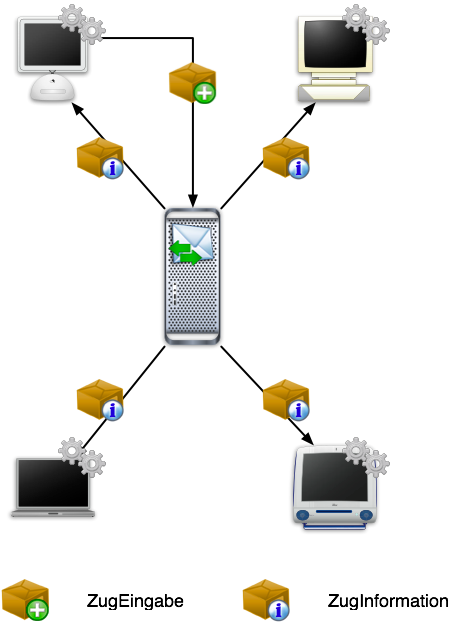
\includegraphics[width=0.6 \textwidth]{client_server}
	\caption{Kommunikation zwischen Client \& Server}
	\label{fig:client_server}
\end{figure}

Die Validierung der gespielten Züge geschieht auf dem Client, der Server ist zuständig für die Koordination des Spielablaufs und für die Kommunikation zwischen den Spielern.

\subsection{Architektonische Ziele \& Einschränkungen} % (fold)
\label{sub:architektonische_ziele_einschraenkungen}
\paragraph{Designentscheidungen}\label{ssub:designentscheidungen} % (fold)
\subparagraph{Zustandsautomat} % (fold)
\label{ssub:zustandsautomat}
Unser Spiel hat einen komplexen Ablauf, sowohl auf der Client- als auch auf der Serverseite. Der grösste Teil der Abläufe wird von Events im Userinterface oder von Netzwerk-Nachrichten ausgelöst. Darum haben wir uns entschlossen, den Spielablauf in einem Zustandsautomaten zu verpacken.

Damit ist es möglich, den Programmablauf, der sonst in komplexem nacheinander aufzurufendem Programmcode verpackt wäre, in verschiedene Klassen auszulagern und den \emph{Gap} zwischen dem Code und den in der Elaboration gezeichneten Zustandsdiagrammen klein zu halten.
% subparagraph zustandsautomat (end)

\subparagraph{Multitier-Architektur des Servers}\label{ssub:multitier_architektur_des_servers} % (fold)
Der Server wurde in mehrere Schichten und vertikal angeordnete Partitions aufgeteilt. Diese Hierarchie hat sich deshalb als erforderlich erwiesen, da sonst Abhängigkeiten von tieferliegenden zu höherliegenden Schichten entstehen würden.
% subparagraph multitier_architektur_des_servers (end)
\subparagraph{Applikationsschicht}\label{ssub:applikationsschicht} % (fold)
Die Applikationsschicht wurde eingeführt, weil es wegen der Netzwerkfähigkeit viel Synchronisationsarbeit (z.\,B. für Zustände) gibt. Sie hat folgende Hauptaufgaben:
	\begin{itemize}
		\item Zustandssynchronisation als erste Vorstufe der Netzwerkkommunikation. Spezifische Nachrichten werden eingepackt, an die darunterliegenden Schichten weitergeleitet, um dann über das Netzwerk verteilt und empfangen zu werden.
		\item Controller-Komponente des MVC-Konzeptes, welche die Ereignisse im UI abfängt und verarbeitet, sowie Änderungen in der Problem-Domain an das UI weiterleitet.
	\end{itemize}
% subparagraph applikationsschicht (end)

% paragraph designentscheidungen (end)
\paragraph{Verwendete Entwicklungswerkzeuge}\label{ssub:verwendete_entwicklungswerkzeuge} % (fold)
Als Entwicklungswerkzeug wird MagicDraw UML verwendet. Es arbeitet Plattformunabhängig (Java), ist einfach handhabbar und hat sehr gute Funktionalitäten zur Code-Generierung. Die erzeugten Dateien lassen sich im XML-Format im SVN-Repository verwalten. Ein Nachteil ist, dass immer nur eine Person gleichzeitig an einem Projekt/Modul arbeiten kann, da MagicDraw UML keine SVN-Integration bietet und Konflikte nicht aufgelöst werden können.
% paragraph verwendete_entwicklungswerkzeuge (end)
\paragraph{Teamstruktur}\label{ssub:teamstruktur} % (fold)
Die Aufteilung des Teams ist aus den Arbeitspaketen in der Excel-Zeiterfassung ersichtlich. Die Verantwortlichkeiten sind in der Analysespezifikation geregelt.
% paragraph teamstruktur (end)
% subsection architektonische_ziele_einschraenkungen (end)

\clearpage
\section{Design Pakete} % (fold)
\label{design_pakete}

\subsection{Logische Sicht} % (fold)
\label{sub:logische_sicht}

\subsubsection{Schichtenarchitektur} % (fold)
\label{sub:schichtenarchitektur}
Für die logische Strukturierung des Projektes wird eine vierschichtige Architektur verwendet, wie in Abbildung~\vref{fig:architektur_schichten} dargestellt. Dabei setzt jede Schicht direkt auf den Diensten der darunterliegenden Schichten auf. Schichten können transparent sein. Dadurch ergeben sich wenige Indirektionen und eine einfache Nutzung der Dienste einer Schicht. Wo möglich und sinnvoll, werden Schnittstellen zwischen Schichten durch eine Fassade gebündelt, um die Kopplung zwischen den Schichten zu verringern. Dadurch lassen sich die Schnittstellen für die Schichten auch klarer definieren und sind einfacher zu nutzen. Im UI wird das MVC-Konzept verwendet, da eine komplexe Darstellungslogik durch das Spiel gegeben ist.
\begin{figure}
	\centering
	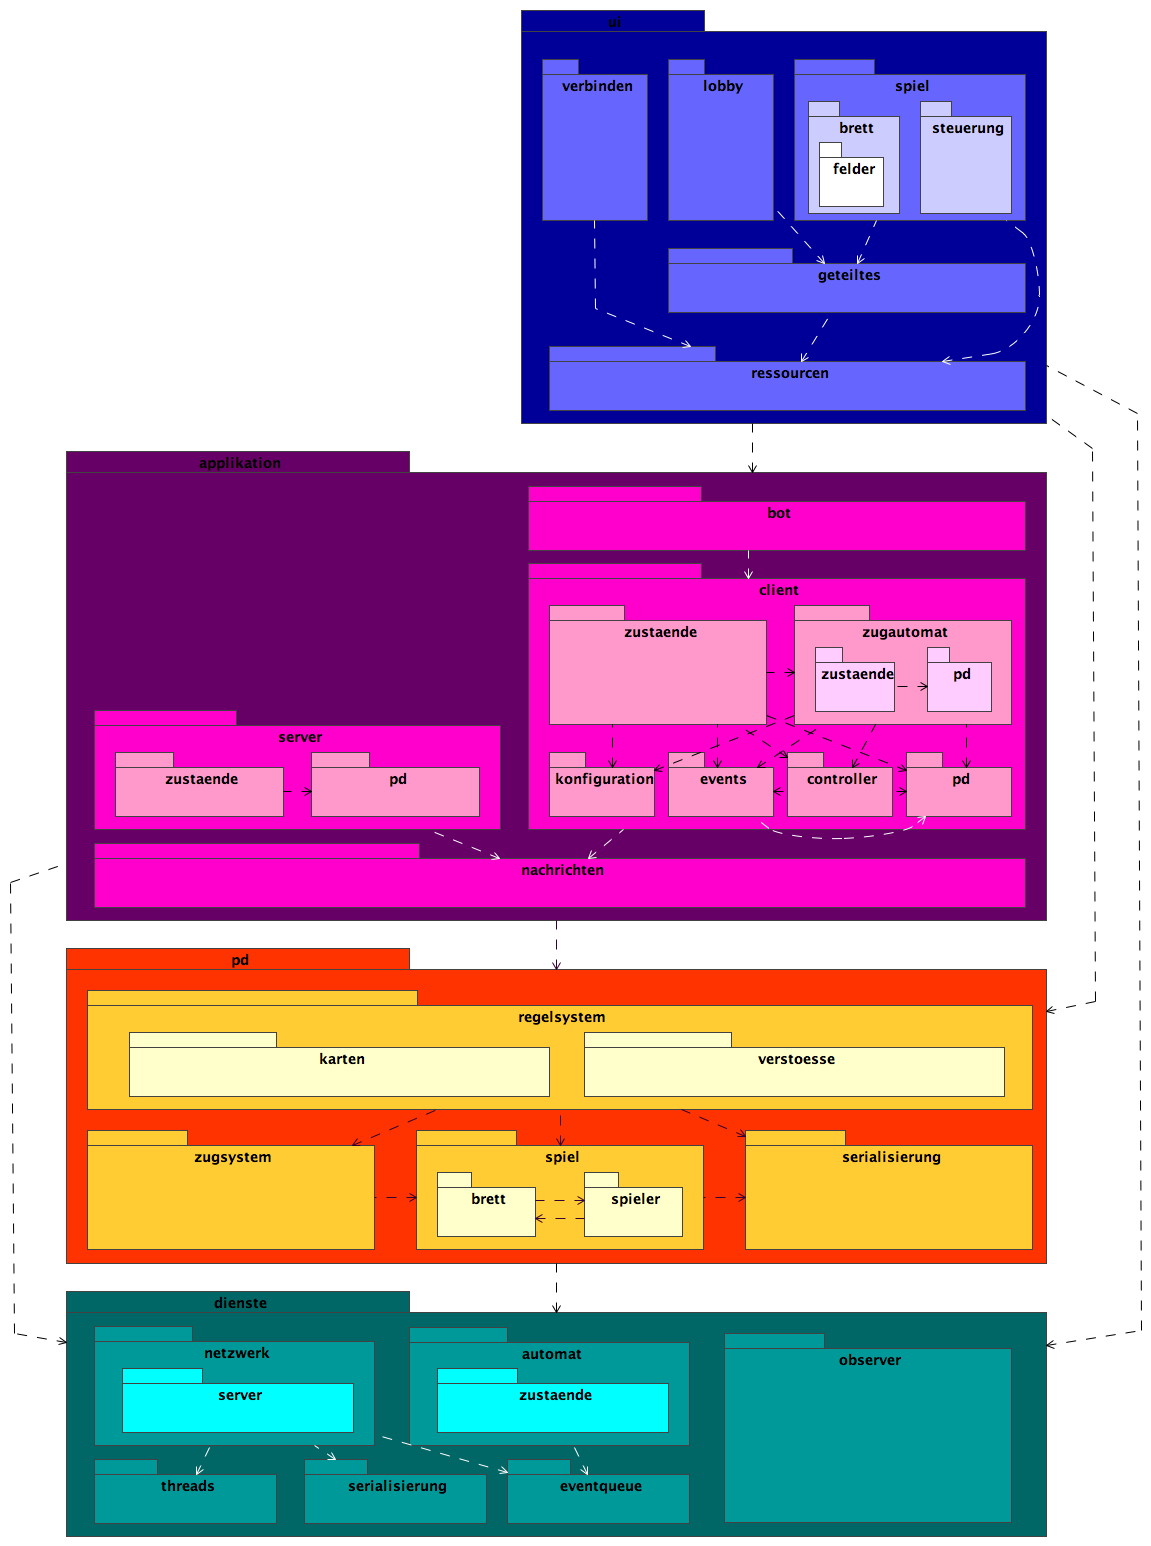
\includegraphics[width=\textwidth]{architektur_schichten}
	\caption{Schichtenarchitektur}
	\label{fig:architektur_schichten}
\end{figure}
\clearpage
\begin{figure}
	\centering
	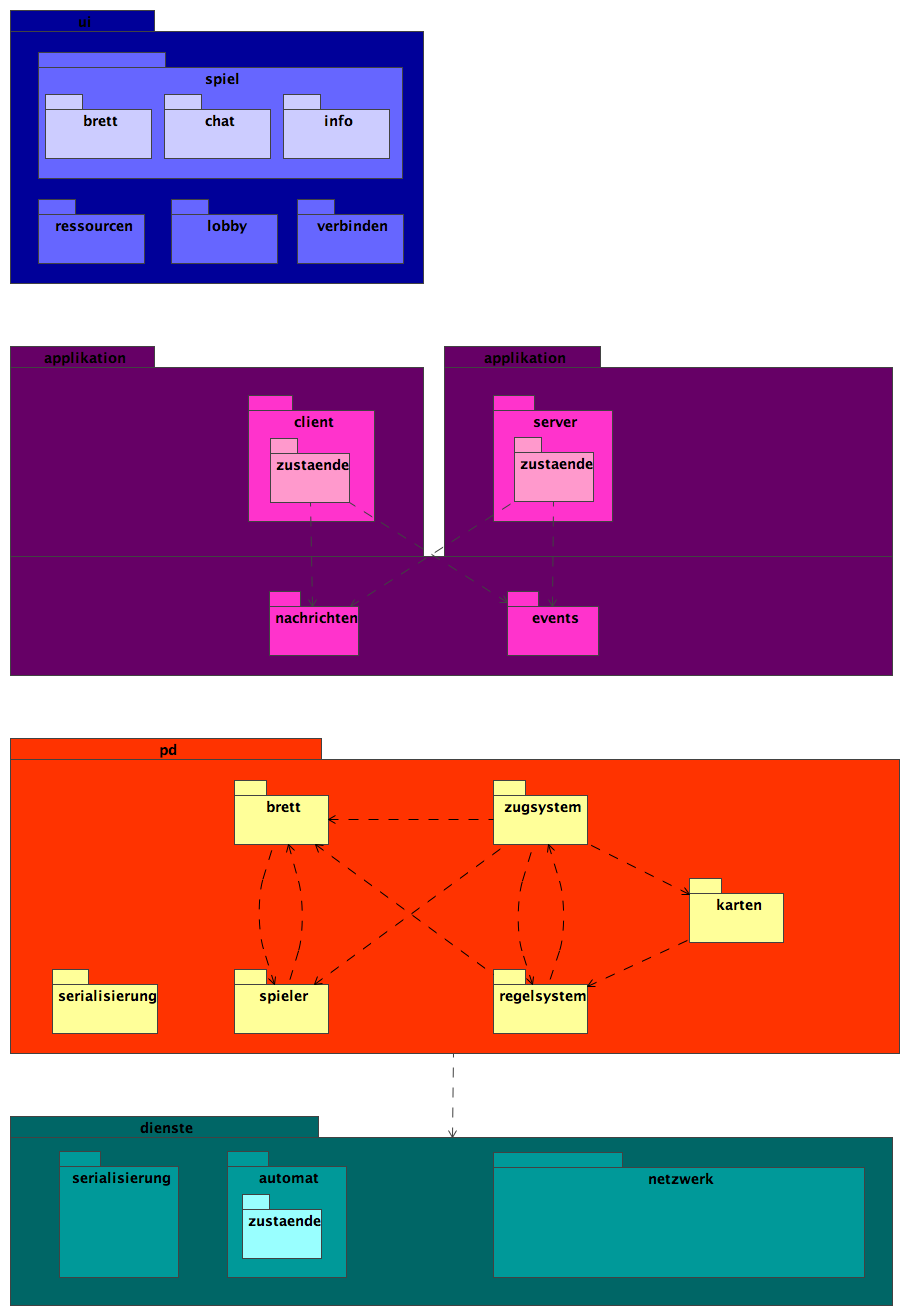
\includegraphics[width=\textwidth]{architektur_partitions}
	\caption{Partitionen in der Architektur}
	\label{fig:architektur_partitions}
\end{figure}
% subsubsection schichtenarchitektur (end)

\clearpage

\subsubsection{Package pd} % (fold)
\label{ssub:package_pd}
\subparagraph{Beschreibung}
In der Problem-Domain-Schicht wird die gesamte Spiellogik gekapselt. Sie wird direkt von der darüberliegenden Applikationsschicht verwendet.

\subparagraph{Schnittstellen} % (fold)
\label{ssub:schnittstellen}
\begin{itemize}
	\item Package pd.zugsystem wird von applikation.zugentgegennahme verwendet, um Züge zu verarbeiten.
\end{itemize}
% subparagraph schnittstellen (end)
% subsubsection package_pd (end)

\subsubsection{Package pd.karten} % (fold)
\label{ssub:package_pd_karten}
\subparagraph{Beschreibung}
Beinhaltet alle Karten, die Kartenfarben, das Deck und den Kartengeber. 

\subparagraph{Schnittstellen} % (fold)
\label{ssub:schnittstellen}
\begin{itemize}
	\item Als Einstiegspunkt für die Karten wird der Kartengeber verwendet, welcher das Mischen und das Ziehen einer Karte vom Stapel bereitstellt.
\end{itemize}
% subparagraph schnittstellen (end)

\begin{figure}[h]
	\centering
	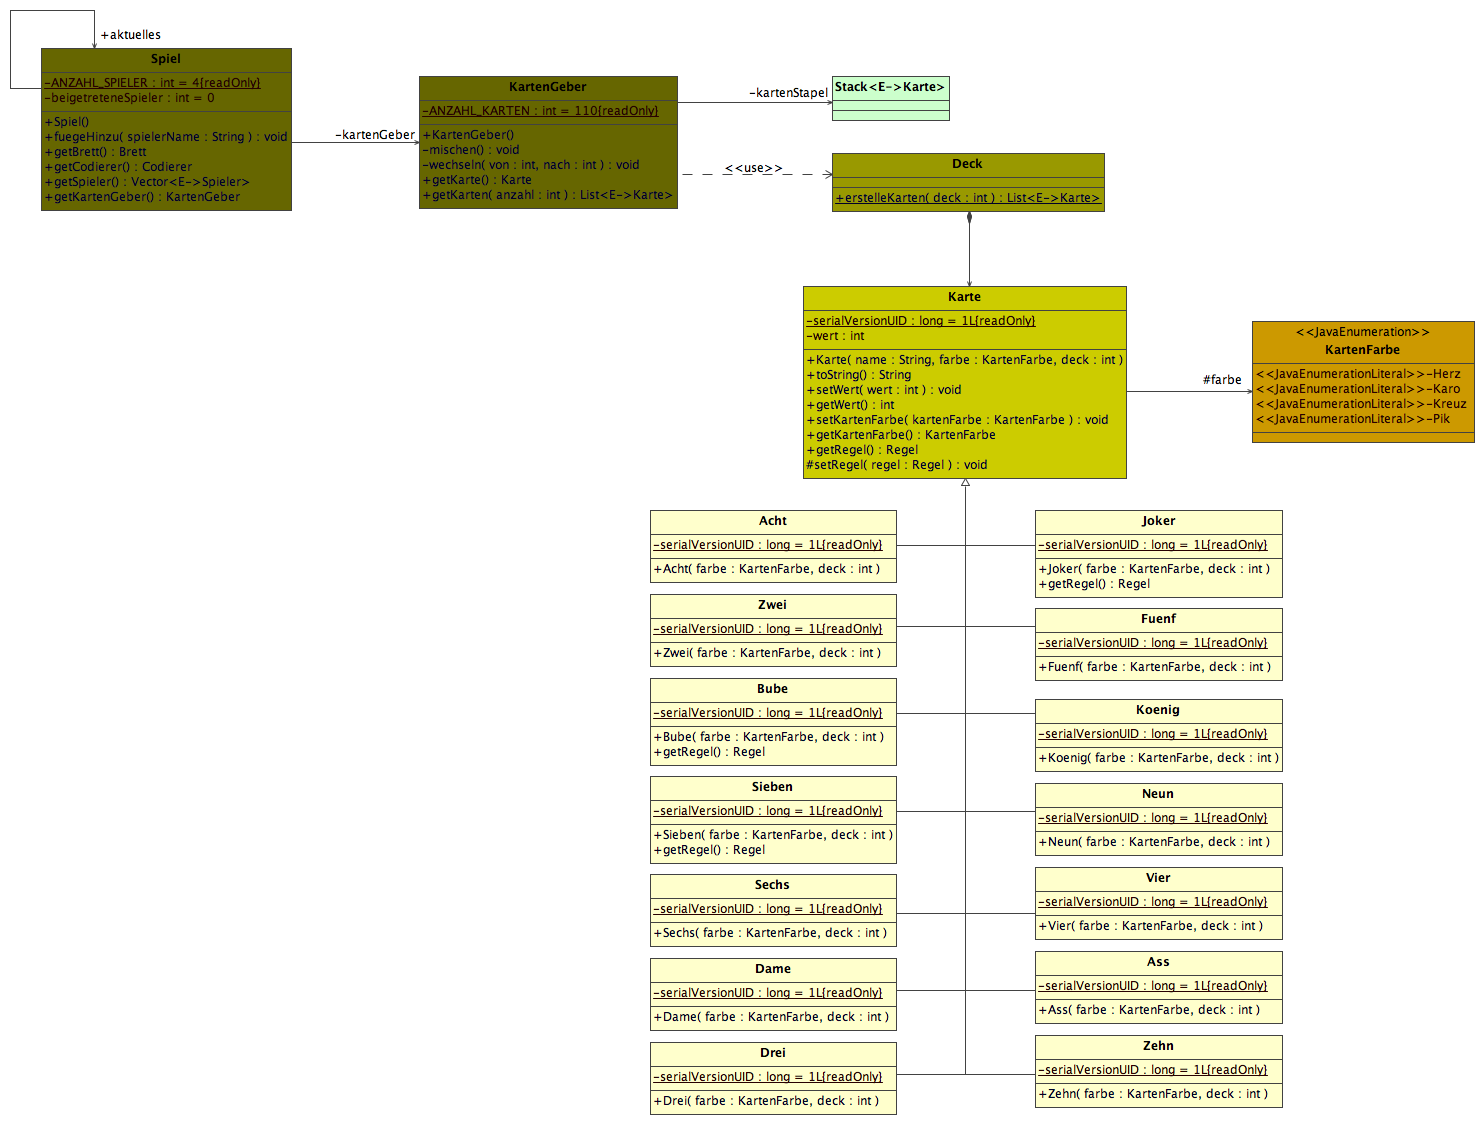
\includegraphics[width=0.8 \textwidth]{pd_kartengeber}
	\caption{Klassendiagramm Kartengeber}
	\label{fig:pd_kartengeber}
\end{figure}

% subsubsection package_pd_karten (end)

\clearpage
\subsubsection{Package pd.regelsystem, pd.zugsystem} % (fold)
\label{ssub:package_pd_regelsystem}
\subparagraph{Beschreibung}
Das Regel- und das Zugsystem sind eng miteinander verbunden. Sie nehmen die Aufgaben der Problem-Domain-Schicht wahr und stellen die Validierung der Züge sicher und berechnet die daraus resultierenden Aktionen in der Problem-Domain (Figur von Feld X auf Feld Y verschieben).

\subparagraph{Schnittstellen} % (fold)
\label{ssub:schnittstellen}
\begin{itemize}
	\item Die Zugeingabe fasst die Informationen zusammen, die für einen Zug benötigt werden und über sie wird validiert, was zu einem ausführbaren Zug führt.
\end{itemize}
% subparagraph schnittstellen (end)

\begin{figure}[h]
	\centering
	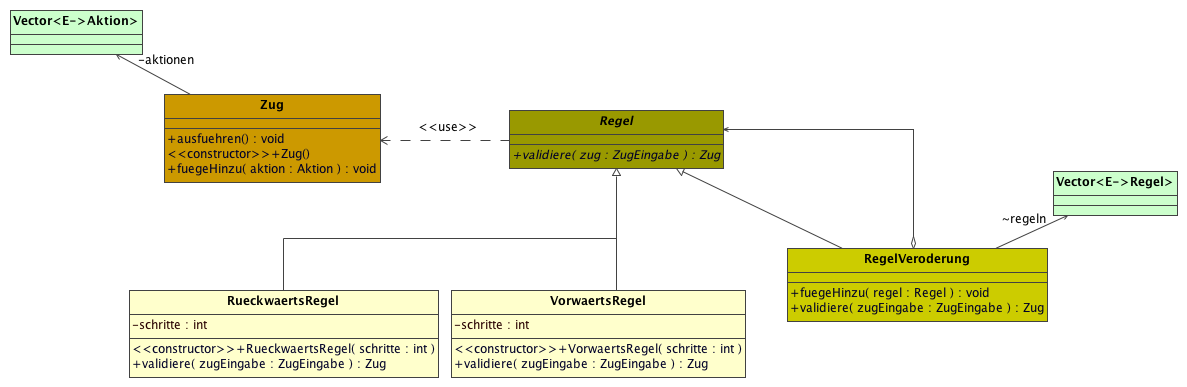
\includegraphics[width=\textwidth]{pd_regelsystem}
	\caption{Klassendiagramm Regelsystem}
	\label{fig:pd_regelsystem}
\end{figure}

% paragraph package_pd_regelsystem (end)

\clearpage
\subsubsection{Package pd.brett, pd.spieler} % (fold)
\label{ssub:package_pd_brett}
\subparagraph{Beschreibung}
Die beiden Packages sind eng miteinander verbunden und stellen die Abstraktion des Bretts (welches die Felder enthält), der Figuren und des Spielers in der Problem-Domain dar.

\subparagraph{Schnittstellen}
\begin{itemize}
	\item Der Einstiegspunkt ist das Spiel, da es das Brett, den Kartengeber und die Spieler enthält.
\end{itemize}

\label{ssub:diagramme}
\begin{figure}[h]
	\centering
	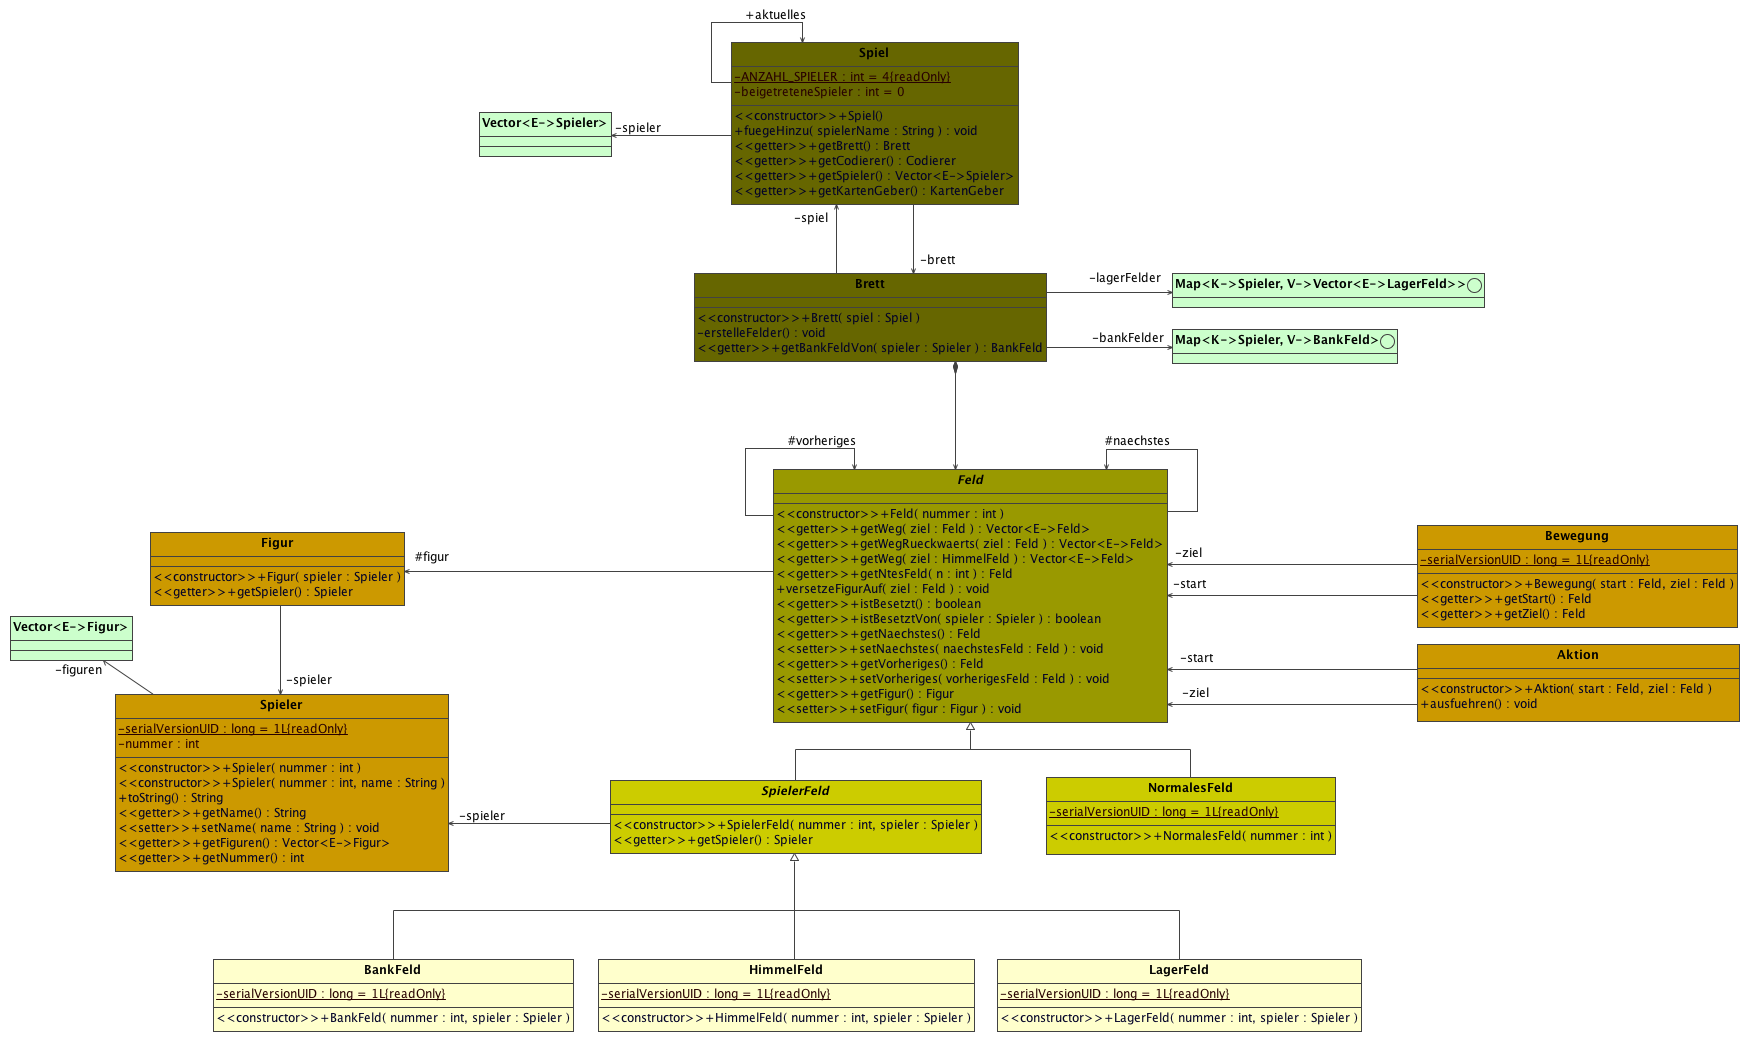
\includegraphics[width=\textwidth]{pd_brett}
	\caption{Klassendiagramm Brett und Figuren}
	\label{fig:pd_brett}
\end{figure}

% paragraph package_pd_brett (end)

\clearpage
\subsubsection{Package pd.serialisierung}

\subparagraph{Beschreibung}
Implementiert die abstrakten Klassen von dienste.serialisierung, um die Serialisierung von Klassen der Problem-Domain zu ermöglichen.

\subparagraph{Schnittstellen}
\begin{itemize}
	\item Bietet eine Basisklasse (BodesuriCodierbaresObjekt) für die Klassen der Problem-Domain an, die serialisiert werden können.
\end{itemize}

\begin{figure}[h]
	\centering
	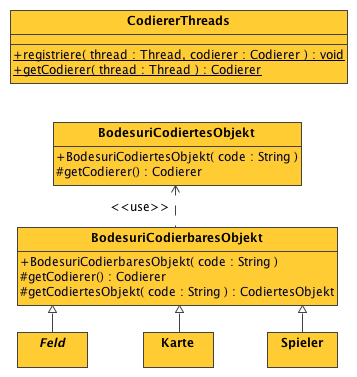
\includegraphics[width=0.5 \textwidth]{kd_pd_serialisierung}
	\caption{Klassendiagramm Serialisierung in PD}
	\label{fig:kd_pd_serialisierung}
\end{figure}

\clearpage
\subsubsection{Package dienste.automat} % (fold)
\label{ssub:package_dienste}
\subparagraph{Beschreibung}
Beinhaltet einen Zustandsautomaten der im Client und im Server eine gezielte Abarbeitung
des Spielablaufs sorgt. Der Automat wechselt aufgrund externer Events auf vorher definierten
Bahnen zwischen den Zuständen hin und her.

\subparagraph{Schnittstellen} % (fold)
\label{ssub:schnittstellen}
\begin{itemize}
	\item Der Automat muss von den darüberliegenden Klassen abgeleitet und spezifisch implementiert werden.
\end{itemize}	
% subparagraph schnittstellen (end)

\begin{figure}[h]
	\centering
	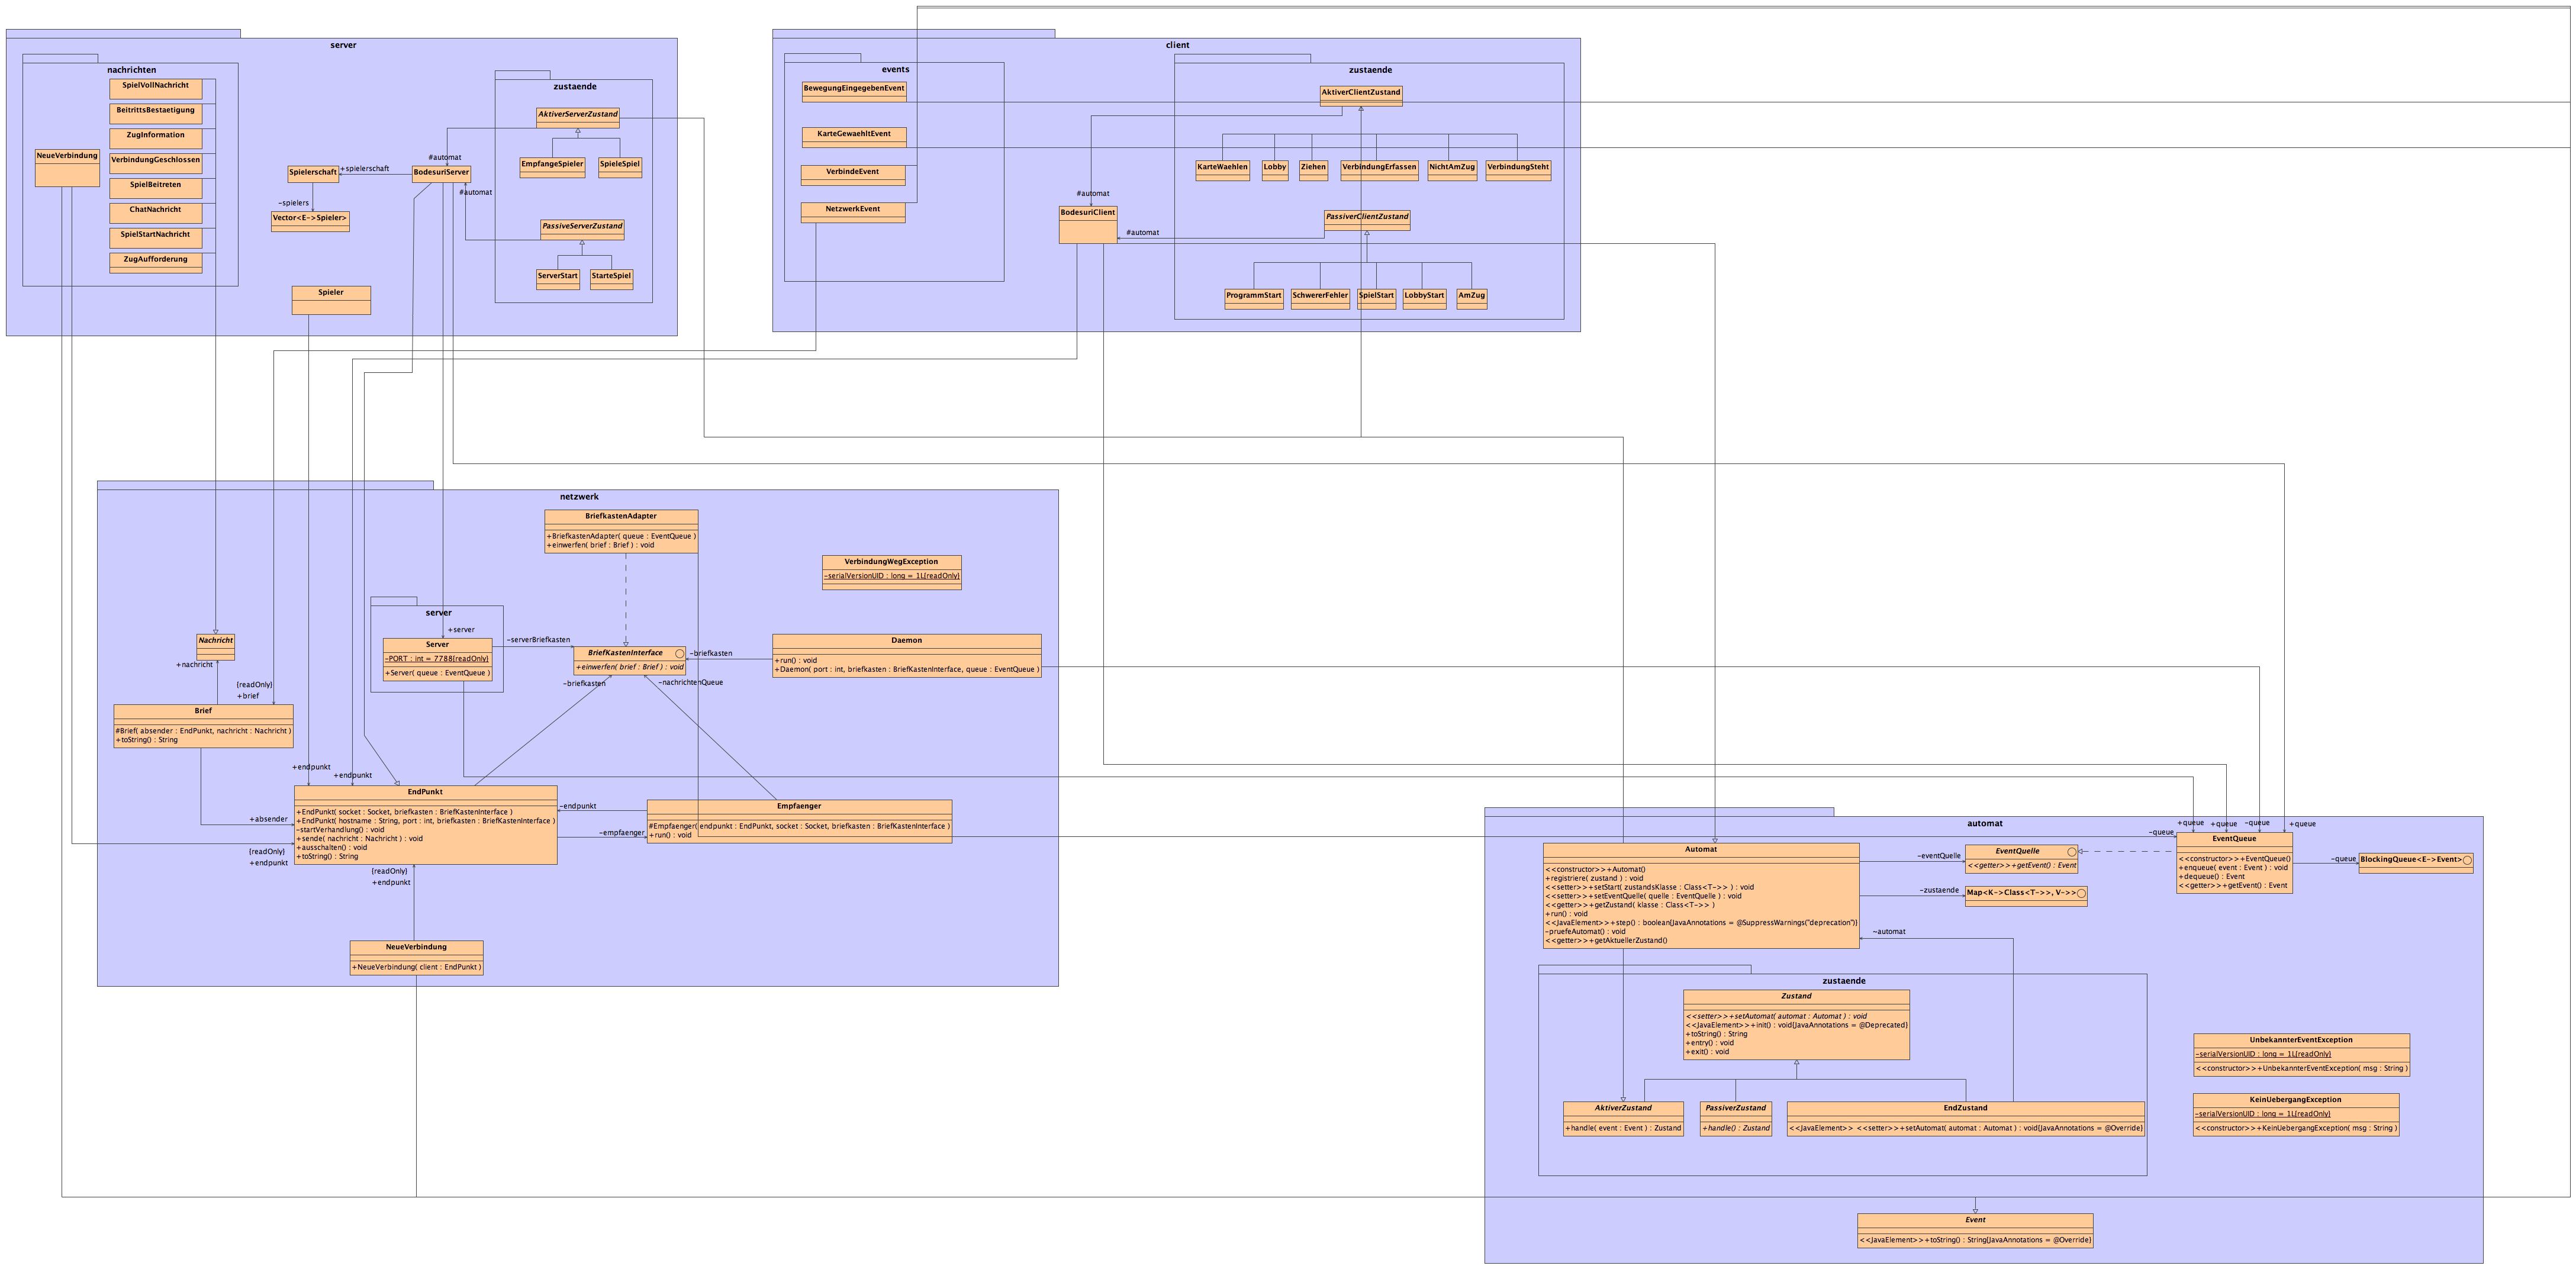
\includegraphics[width=\textwidth]{dienste_automat_klassendiagramm}
	\caption{Klassendiagramm Automat}
	\label{fig:dienste_serialisierung}
\end{figure}

% paragraph package_automat (end)

\clearpage
\subsubsection{Package dienste.serialisierung}

\subparagraph{Beschreibung}
Dieses Package ist für die Serialisierung und Deserialisierung der Java-Objekte zuständig, welche anschliessend über das Netzwerk versendet werden.

\subparagraph{Schnittstellen}
\begin{itemize}
	\item Die abstrakte Klasse CodierbaresObjekt muss vom Benutzer dieses Packages implementiert werden. Dabei müssen die Methoden getCodierer() und getCodiertesObjekt() überschrieben werden. getCodiertesObjekt() sollte ein neues konkretes CodiertesObjekt (z.\,B. BodesuriCodiertesObjekt) erstellen.
	\item Die zweite abstrakte Klasse CodiertesObjekt muss auch implementiert werden. Dort muss nur getCodierer() überschrieben werden, welches den gleichen Codierer zurückgeben sollte, wie bei CodierbaresObjekt.
\end{itemize}

\begin{figure}[h]
	\centering
	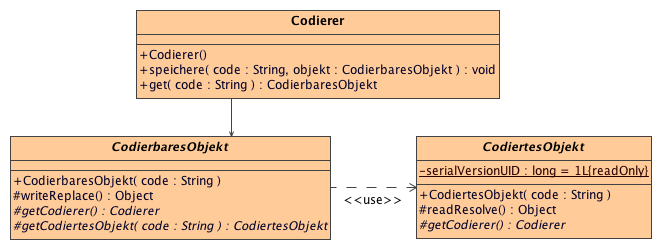
\includegraphics[width=\textwidth]{kd_dienste_serialisierung}
	\caption{Klassendiagramm Serialisierung in Dienste}
	\label{fig:kd_dienste_serialisierung}
\end{figure}

\clearpage
\subsubsection{Package dienste.netzwerk} % (fold)
\label{ssub:package_dienste_netzwerk}
\subparagraph{Beschreibung}
Dieses Package kapselt die Socket-Schnittstelle von Java und bietet Dienste für die Netzwerkkommunikation an.

\subparagraph{Schnittstellen} % (fold)
\label{ssub:schnittstellen}
\begin{itemize}
	\item dienste.netzwerk verwendet die Klassen Event und EventQueue für die Kommunikation mit den darüberliegenden Schichten.
	\item Die Kommunikation mit dem Netzwerk findet über die Bibliotheken java.net statt.
\end{itemize}

\begin{figure}[h]
	\centering
	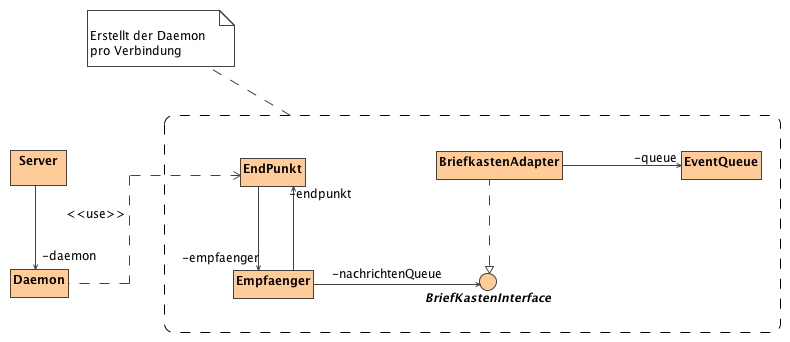
\includegraphics[width=0.9 \textwidth]{dienste_netzwerk_client}
	\caption{Klassendiagramm Client in Netzwerk}
	\label{fig:dienste_netzwerk_client}
\end{figure}

\begin{figure}[h]
	\centering
	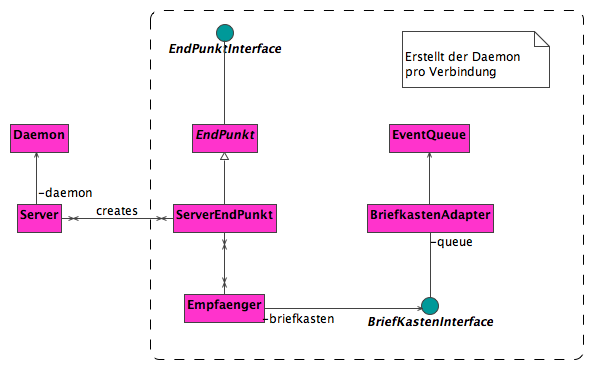
\includegraphics[width=0.9 \textwidth]{dienste_netzwerk_server}
	\caption{Klassendiagramm Server in Netzwerk}
	\label{fig:dienste_netzwerk_server}
\end{figure}

% subparagraph schnittstellen (end)
% paragraph package_dienste_netzwerk (end)

\clearpage
\subsubsection{Package ui} % (fold)
\label{ssub:package_ui}
Die UI-Schicht ist für die graphische Darstellung verantwortlich. Sie kommuniziert mit der Applikationsschicht top-down über direkte Assoziationen und bottom-up über Observer.
% subparagraph beschreibung (end)
% paragraph package_ui (end)

\begin{description}
	\item[ui.lobby] Ist für die Darstellung der Lobby verantwortlich.
	\item[ui.ressourcen] Es beinhaltet die Ressourcen, die für das Optische benötigt werden.
	\item[ui.spiel] Wird verwendet um die Views des Spieles zusammenzuführen.
	\item[ui.spiel.brett] Kümmert sich um die Darstellung des Brettes.
	\item[ui.spiel.chat] Dient zur Kommunikation für die einzelnen Spieler untereinander.
	\item[ui.spiel.info] Stellt die View dar, das die Spielerinfos beinhaltet.
	\item[ui.verbinden] Dienst zur Erstellung der Verbindung mit dem Server.
\end{description}

\begin{figure}[h]
	\centering
	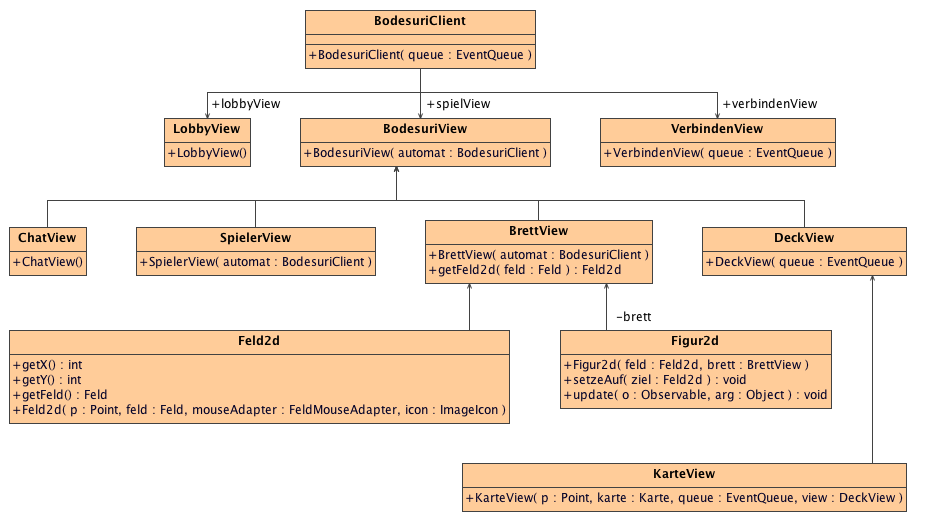
\includegraphics[width=\textwidth]{ui_alle}
	\caption{Klassendiagramm UI}
	\label{fig:ui_alle}
\end{figure}

\clearpage
\subsubsection{Package applikation} % (fold)
\label{ssub:package_applikation}
\subparagraph{Beschreibung}
Die Applikationsschicht ist für die Zustandssynchronisation (Spielstände usw.) verantwortlich.

\subsubsection{Package applikation.zugentgegennahme} % (fold)
\label{ssub:package_applikation_zugentgegennahme}
\subparagraph{Beschreibung}
\label{ssub:beschreibung}
Die Zugentgegennahme sorgt für die Verbindung vom UI zur Problem-Domain. Durch das Klicken (ziehen der Figur) im UI werden Züge an die Problem-Domain weitergeleitet und die Validierung eingeleitet.
% subparagraph beschreibung (end)

\subparagraph{Schnittstellen} % (fold)
\label{ssub:schnittstellen}
\begin{itemize}
	\item Bietet die Methode ziehen() an, welche die Zugentgegennahme in einen neuen Status versetzt.
\end{itemize}
% subparagraph schnittstellen (end)

\begin{figure}[h]
	\centering
	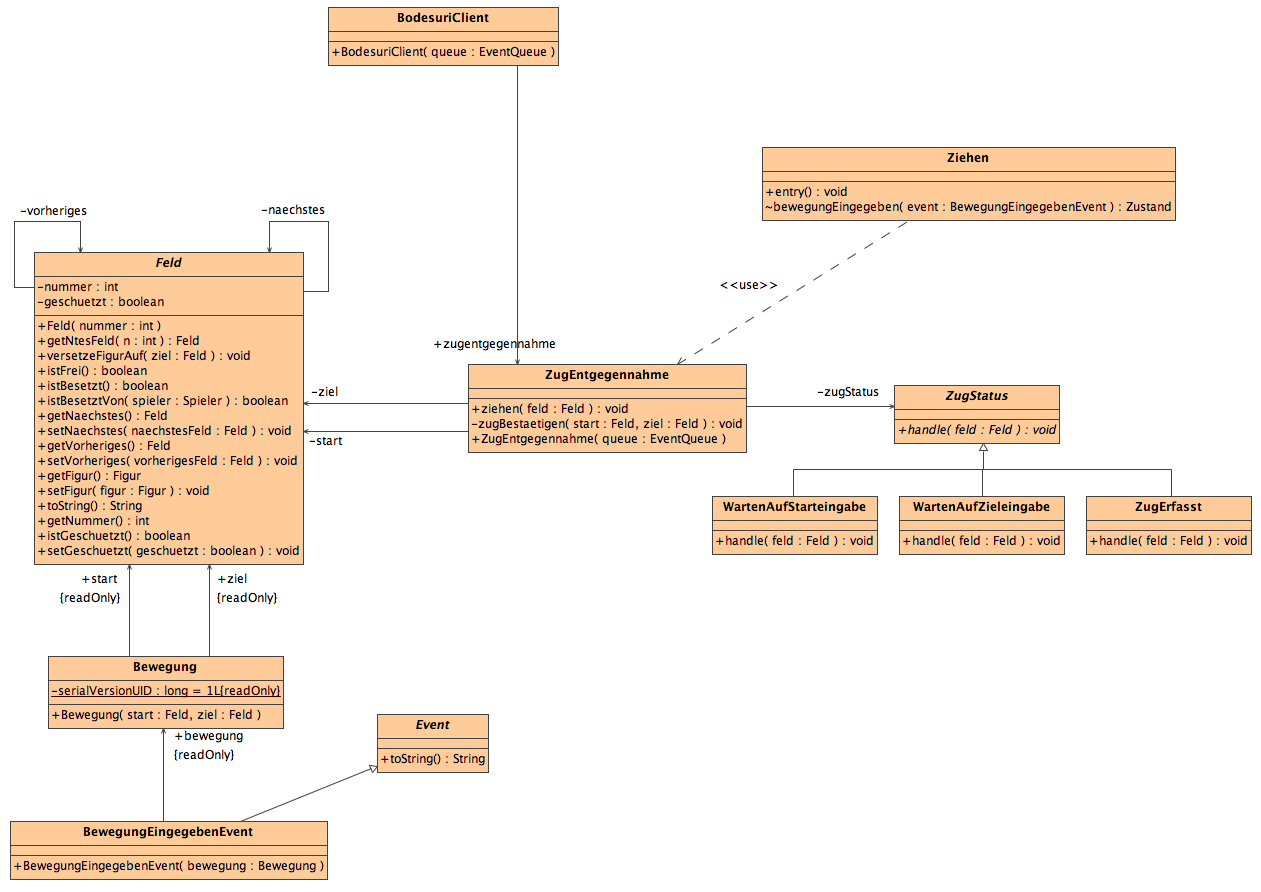
\includegraphics[width=\textwidth]{applikation_zugentgegennahme}
	\caption{Klassendiagramm Zugentgegennahme}
	\label{fig:applikation_zugentgegennahme}
\end{figure}

% paragraph package_applikation_zugentgegennahme (end)

\clearpage
\subsubsection{Package applikation.client}
\label{ssub:package_applikation_client} % (fold)
\subparagraph{Beschreibung}
\label{ssub:beschreibung}
Der Zustandsautomat des Clients und dessen Zustände. Sorgt für den korrekten Ablauf des Spiels auf der Client-Seite. Verarbeitet die eintretenden Events von GUI und Netzwerk und löst entsprechende Aktionen aus.
% subparagraph beschreibung (end)

\subparagraph{Schnittstellen}
\label{ssub:schnittstellen}
\begin{itemize}
	\item Bietet verschiedenste Instanzvariablen für das GUI und die zum Server gehörenden Zustände an.
\end{itemize}
% subparagraph schnittstellen (end)

\begin{figure}[h]
	\centering
	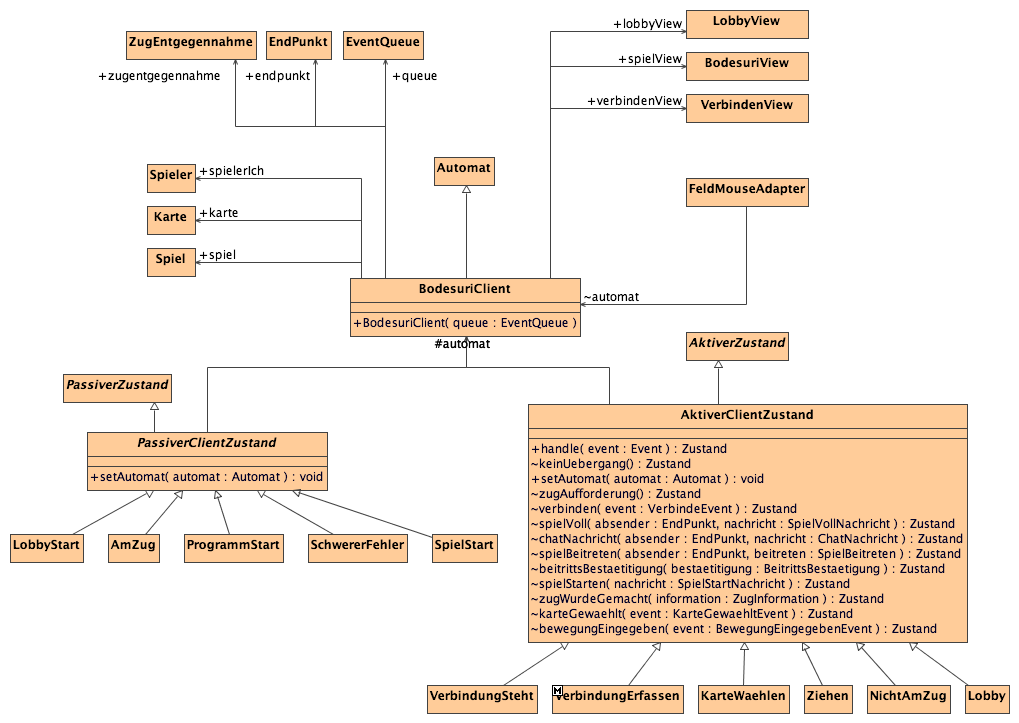
\includegraphics[width=\textwidth]{kd_applikation_client}
	\caption{Klassendiagramm Client in Applikation}
	\label{fig:kd_applikation_client}
\end{figure}
% subsubsection package_applikation_client (end)

\clearpage
\subsubsection{Package applikation.server}
\label{ssub:package_applikation_server} % (fold)
\subparagraph{Beschreibung}
\label{ssub:beschreibung}
Der Zustandsautomat des Servers und dessen Zustände. Sorgt für den korrekten Ablauf des Spiels auf der Server-Seite. Verarbeitet die eintretenden Events vom Netzwerk und löst entsprechende Aktionen aus, um den Spielablauf zu steuern.
% subparagraph beschreibung (end)

% subsubsection package_applikation_server (end)

\begin{figure}[h]
	\centering
	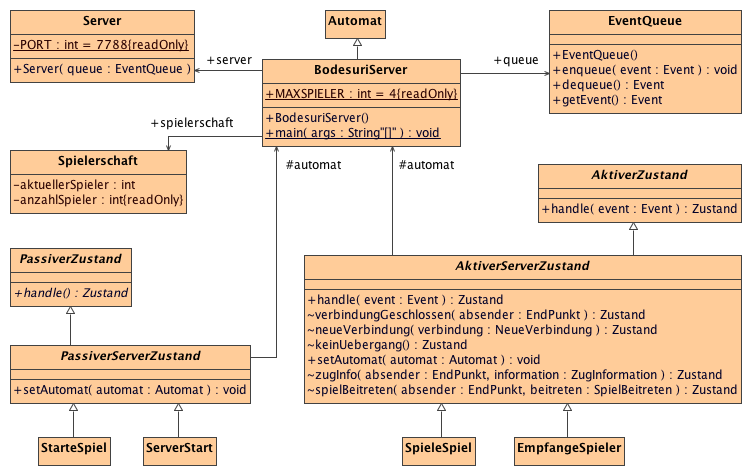
\includegraphics[width=\textwidth]{kd_applikation_server}
	\caption{Klassendiagramm Server in Applikation}
	\label{fig:kd_applikation_server}
\end{figure}

\clearpage
\subsubsection{Package applikation.events}
\label{ssub:package_applikation_events}
\subparagraph{Beschreibung}
\label{ssub:beschreibung}
Dieses Package beinhaltet die Events, die eintreten können und um deren Behandlung sich der Automat kümmert.
\begin{figure}[h]
	\centering
	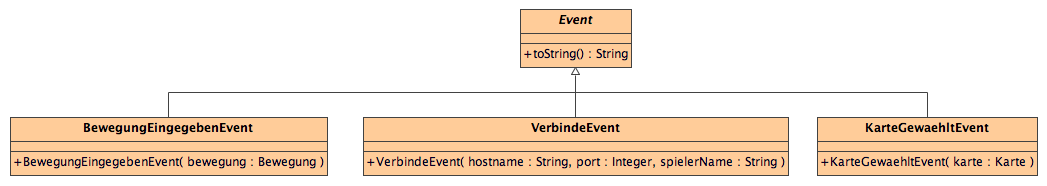
\includegraphics[width=\textwidth]{kd_applikation_events}
	\caption{Klassendiagramm Events}
	\label{fig:kd_applikation_events}
\end{figure}

\subsubsection{Package applikation.nachrichten}
\label{ssub:package_applikation_nachrichten}
\subparagraph{Beschreibung}
\label{ssub:beschreibung}
Dieses Package beinhaltet alle möglichen Nachrichtentypen, die zur Kommunikation zwischen Client und Server verwendet werden.
\begin{figure}[h]
	\centering
	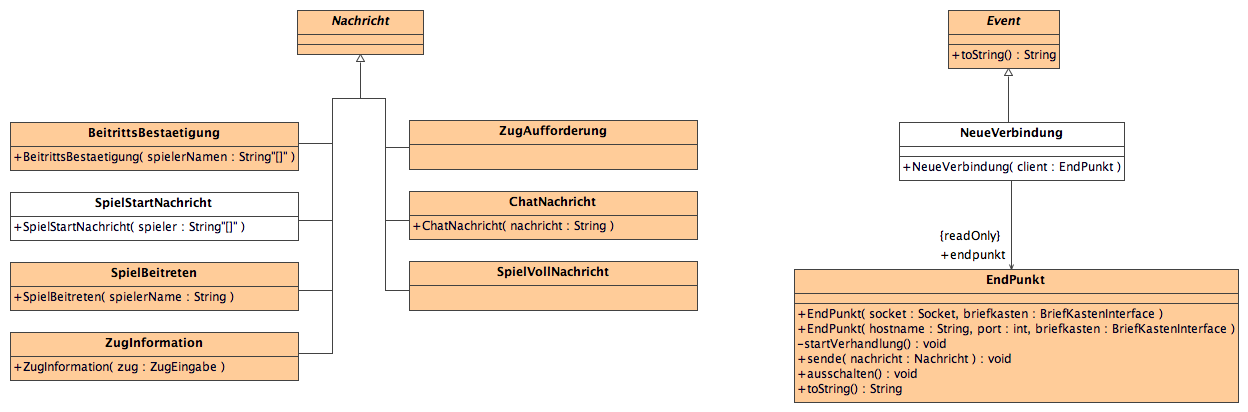
\includegraphics[width=\textwidth]{kd_applikation_nachricht}
	\caption{Klassendiagramm Nachrichten}
	\label{fig:kd_applikation_nachricht}
\end{figure}
\clearpage

\subsection{Prozesse \& Threads} % (fold)
\label{sub:prozesse_threads}

Ein reguläres Bodesuri-Spiel besteht aus fünf eigenständigen Komponenten. Dies sind die vier Clients und der zentrale Server. Die Clients kommunizieren über je einen TCP-Socket mit dem Server.

\begin{figure}[h]
	\centering
	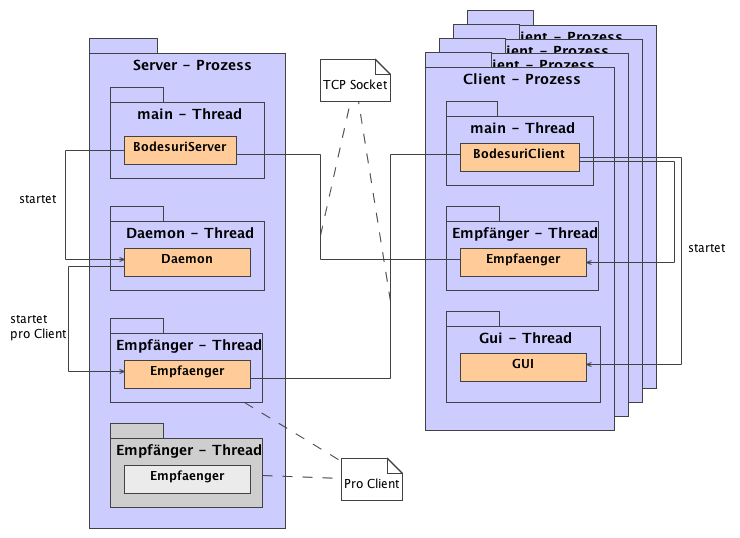
\includegraphics[width=\textwidth]{prozesse_und_threads}
	\caption{Prozesse \& Threads}
	\label{fig:prozesse_und_threads}
\end{figure}

\clearpage
\subsubsection{Client-Threads} % (fold)
\label{ssub:client_threads}

% subsubsection client_threads (end)

\paragraph{Main-Thread} % (fold)
\label{ssub:main_thread}

Der Main-Thread des Clients ist für die geordnete Koordination zwischen dem Spieler (via GUI) und den anderen Clients (via Server) zuständig.


\begin{tabular}{@{} l p{12.5cm}}
\textbf{Klasse}       & BodesuriClient \\
\textbf{Anzahl}       & 1 \\
\textbf{Gestartet}    & Bei Prozessbeginn \\
\textbf{Beendet}      & Bei Programmende
\end{tabular}

% paragraph main_thread (end)

\paragraph{Empfänger-Thread} % (fold)
\label{ssub:empfänger_thread}

Der Empfänger-Thread ist für den Empfang von Netzwerk-Nachrichten zuständig. Er liest aus einem java.net.Socket und speichert die eingegangenen Nachrichten über das Briefkasten-Interface in der EventQueue.

\begin{tabular}{@{} l p{12.5cm}}
\textbf{Klasse}       & Empfaenger \\
\textbf{Anzahl}       & 1 \\
\textbf{Gestartet}    & Bei Verbindungsaufbau durch den Main-Thread (Klasse Endpunkt) \\
\textbf{Beendet}      & Bei Verbindungsabbau durch den Main-Thread (Klasse Endpunkt)
\end{tabular}

% paragraph empfänger_thread (end)

\paragraph{Timer(s)} % (fold)
\label{ssub:timer_s_}

Timer werden an verschiedenen Stellen für das Timeout-Handling eingesetzt. Sie werden bei Bedarf gestartet und lösen nach einer definierten Zeitspanne einen Event aus bzw. werden vom Anwender wieder gestoppt.

\begin{tabular}{@{} l p{12.5cm}}
\textbf{Klasse}       & Timer \\
\textbf{Anzahl}       & 0..* \\
\textbf{Gestartet}    & Bei Bedarf durch den Main-Thread \\
\textbf{Beendet}      & Entweder durch sich selber wenn der Timer ablief oder auf Anweisung des Main-Threads wenn der Timer nicht mehr benötigt wird. 
\end{tabular}

% paragraph timer_s_ (end)

\paragraph{Swing-Threads} % (fold)
\label{ssub:swing_threads}

Swing startet intern verschiedene Threads. Die genauen Abläufe und Struktur dieser Threads sind für dieses Projekt nicht relevant.

\begin{tabular}{@{} l p{12.5cm}}
\textbf{Klasse}       & AWK-AppKit \\
\textbf{Anzahl}       & 1..* \\
\textbf{Gestartet}    & Durch Swing \\
\textbf{Beendet}      & N/A
\end{tabular}

% paragraph swing_threads (end)

\clearpage
\subsubsection{Server Threads} % (fold)
\label{ssub:server}

Der Server ist für die Koordination der einzelnen Clients zuständig.

\begin{tabular}{@{} l p{12.5cm}}
\textbf{Klasse}       & BodesuriServer \\
\textbf{Anzahl}       & 1 \\
\textbf{Gestartet}    & bei Prozessbeginn \\
\textbf{Beendet}      & Bei Spielende oder bei schweren Fehlern
\end{tabular}

% subsubsection server (end)

\paragraph{Daemon} % (fold)
\label{ssub:daemon}

Der Daemon ist ein Teil des Servers. Er nimmt eingehende Verbindungen entgegegen und meldet diese über das BriefkastenInterface (via EventQueue) an den Nutzer des Servers.

\begin{tabular}{@{} l p{12.5cm}}
\textbf{Klasse}       & Daemon \\
\textbf{Anzahl}       & 1 \\
\textbf{Gestartet}    & Durch den Main-Thread (Klasse Server) gestartet \\
\textbf{Beendet}      & Bei Programmende
\end{tabular}

% paragraph daemon (end)

\paragraph{Empfänger-Thread} % (fold)
\label{ssub:empfänger_thread}

Der Empfänger-Thread ist für den Empfang von Netzwerk-Nachrichten zuständig. Er liest aus einem java.net.Socket und speichert die eingegangenen Nachrichten über das Briefkasten-Interface in der EventQueue.

\begin{tabular}{@{} l p{12.5cm}}
\textbf{Klasse}       & Empfänger \\
\textbf{Anzahl}       & 1..4 \\
\textbf{Gestartet}    & Durch den Daemon bei eingehenden Verbindungen  \\
\textbf{Beendet}      & Bei Verbindungsabbau durch den Main-Thread
\end{tabular}

% subsection prozesse_threads (end)

\clearpage
\section{Spielablauf \& -zustände} % (fold)
\label{spielzustaende_nachrichten}
\subsection{Zustände Client} % (fold)
\label{sub:zustände_client}
\begin{figure}[h]
	\centering
	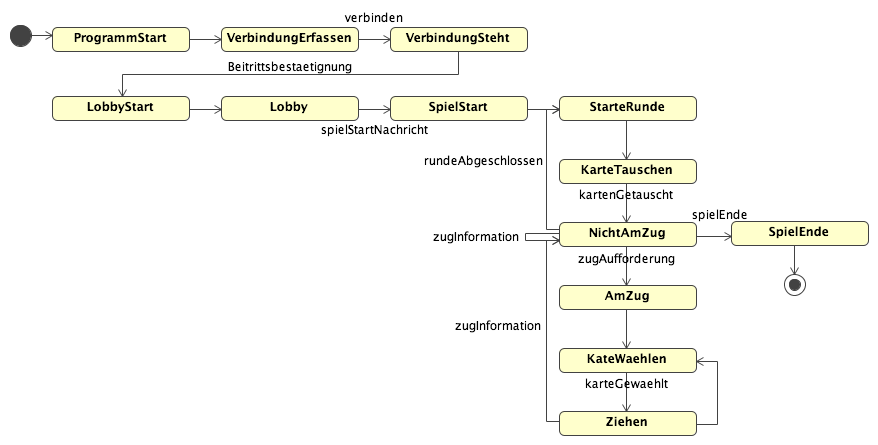
\includegraphics[width=\textwidth]{zd_applikation_bodesuriclient}
	\caption{Zustandsdiagramm Client}
	\label{fig:zd_applikation_bodesuriclient}
\end{figure}

\subsubsection{ProgrammStart} % (fold)
\label{ssub:programmstart}
Zustand in welchem der Automat beim Start ist. Öffnet den VerbindenView und geht direkt in den Zustand VerbindungErfassen über.
% subsubsection programmstart (end)

\subsubsection{VerbindungErfassen} % (fold)
\label{ssub:verbinungerfassen}
Zustand wenn der Spieler die Verbindungsdaten eingeben muss. Wenn ein VerbindeEvent eintrifft wird der Zustand VerbindungSteht aufgerufen.
% subsubsection verbinungerfassen (end)

\subsubsection{VerbindungSteht} % (fold)
\label{ssub:verbindungsteht}
Zustand wenn der Client auf die BeitrittsBestaetigung vom Server wartet. Wenn sie eintrifft wir der Zustand LobbyStart aufgerufen.
% subsubsection verbindungsteht (end)

\subsubsection{LobbyStart} % (fold)
\label{ssub:lobbystart}
Zustand in welchem die Lobby (LobbyView) gestartet wird. Geht direkt in Lobby über.
% subsubsection lobbystart (end)

\subsubsection{Lobby} % (fold)
\label{ssub:lobby}
Zustand wennn der Spieler in der Lobby ist. Wenn eine SpielStartNachricht eintrifft, wird der Zustand SpielStart aufgerufen.
% subsubsection lobby (end)

\subsubsection{SpielStart} % (fold)
\label{ssub:spielstart}
Zustand in welchem das Spiel (BodesuriView) gestartet wird. Geht direkt in StarteRunde über.
% subsubsection spielstart (end)

\subsubsection{StarteRunde} % (fold)
\label{ssub:starterunde}
Zustand in welchem eine neue Runde beginnt. Zeigt die Karten an und geht in den Zustand KarteTauschen über.
% subsubsection starterunde (end)

\subsubsection{KarteTauschen} % (fold)
\label{ssub:kartetauschen}
Zustand in welchem der Client wartet bis der Spieler gewählt hat, welche Karte er seinem Mitspieler geben will und die Karte vom Mitspieler erhält. Geht in den Zustand NichtAmZug über.
% subsubsection kartetauschen (end)

\subsubsection{NichtAmZug} % (fold)
\label{ssub:nichtamzug}
Zustand wenn der Spieler nicht am Zug ist.
\begin{itemize}
	\item Wenn eine ZugAufforderung eintrifft wird der Zustand AmZug aufgerufen.
	\item Wenn eine ZugInformation eintrifft wird der Zug ausgeführt, der Zustand aber nicht gewechselt.
	\item Wenn ein RundeAbgeschlossenEvent eintrifft wird der Zustand StarteRunde aufgerufen.
	\item Wenn eine SpielEnde eintrifft wird der Zustand SpielEnde aufgerufen.
\end{itemize}
% subsubsection nichtamzug (end)

\subsubsection{AmZug} % (fold)
\label{ssub:amzug}
Zustand in welchem der Spieler zum Zug kommt. Geht direkt in KarteWaehlen über.
% subsubsection amzug (end)

\subsubsection{KarteWaehlen} % (fold)
\label{ssub:kartewaehlen}
Zustand wenn der Spieler eine Karte auswählen muss. Wenn der KarteGewaehltEvent eintritt, wird der Zustand Ziehen aufgerufen.
% subsubsection kartewaehlen (end)

\subsubsection{Ziehen} % (fold)
\label{ssub:ziehen}
Zustand wenn der Spieler eine Bewegung machen muss. Wenn ein BewegungEingegebenEvent eintrifft wird der gesamte Zug validiert und der Zustand NichtAmZug aufgerufen.
% subsubsection ziehen (end)

\subsubsection{SpielEnde} % (fold)
\label{ssub:spielende}
Der letzte Zustand des Automaten. Zeigt den Gewinner an und geht in den EndZustand über.
% subsubsection spielende (end)

\subsection{Zustände Server} % (fold)
\label{sub:zustände_server}

Abbildung~\vref{fig:zd_applikation_bodesuriserver} zeigt den Ablauf der Zustände des Servers.

\begin{figure}[h]
	\centering
	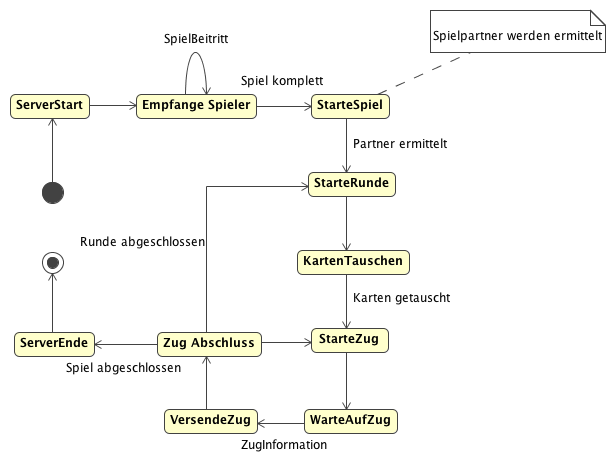
\includegraphics[width=\textwidth]{zd_applikation_bodesuriserver}
	\caption{Zustandsdiagramm Server}
	\label{fig:zd_applikation_bodesuriserver}
\end{figure}

\subsubsection{ServerStart} % (fold)
\label{ssub:serverStart}
Server wird gestartet. Der TCP-Daemon wird initialisiert und es werden die notwenigen Vorbereitungen getroffen um Spieler zu akzeptieren.

% subsubsection spielstart (end)

\subsubsection{EmpfangeSpieler} % (fold)
\label{ssub:empfangespieler}
Neue Spieler können mittels der Nachricht SpielBeitreten dem Spiel beitreten. Dem beigetretenen Spieler wird mit der Nachricht BeitrittBestätigung der Beitritt bestätigt.

Sobald alle Spieler komplett sind, wird in den Zustand StarteSpiel gewechselt.

% subsubsection empfangespieler (end)

\subsubsection{StarteSpiel} % (fold)
\label{ssub:startespiel}
Den Spielern wird der Spielstart mit der Nachricht SpielStart angekündet. Die Partnerschaften werden, wie auf Abbildung~\vref{fig:dienste_partner} gezeigt, zwischen den Spielern ausgehandelt.

% subsubsection startespiel (end)

\subsubsection{StartRunde} % (fold)
\label{ssub:startrunde}
Eine neue Runde wird gestartet und mit der Nachricht RundenStart den Spielern mitgeteilt. Es werden allen Spielern Karten ausgeteilt.

% subsubsection startrunde (end)

\subsubsection{KartenTauschen} % (fold)
\label{ssub:kartentauschen}
Alle Spieler müssen mit ihrem Partner eine Karte tauschen. Der Server wartet bis alle Spieler die zu tauschende Karte mit der Nachricht KartenTausch gemeldet haben. Anschliessend wird die getauschte Karte mit derselben Nachricht dem Partner gemeldet.

% subsubsection kartentauschen (end)

\subsubsection{StarteZug} % (fold)
\label{ssub:startezug}
Ein Zug wird gestartet. Der Server bestimmt welcher Spieler an der Reihe ist und teilt ihm dies mit der Nachricht Zugaufforderung mit. 

% subsubsection startezug (end)

\subsubsection{WarteAufZug} % (fold)
\label{ssub:warteaufzug}
Der Server wartet, bis der Spieler seinen Zug erfasst hat. Sobald dieser mitgeteilt wurde, wechselt der Server in den Zustand VersendeZug.
% subsubsection warteaufzug (end)

\subsubsection{SendeZug} % (fold)
\label{ssub:sendezug}
Der erfasste Zug wird auf Richtigkeit geprüft und anschliessend allen Spielern mitgeteilt.

% subsubsection sendezug (end)

\subsubsection{ZugAbschluss} % (fold)
\label{ssub:zugabschluss}
Server schliesst den Zug formell ab. Es wird geprüft, ob das Spiel beziehungsweise die Runde abgeschlossen ist und in den Zustand SpielEnde respektive RundenStart gewechselt. Ist weder das Spiel noch die Runde fertig wird in den Zustand StartZug gewechselt.

\subsubsection{Spielende} % (fold)
\label{ssub:spielende}
Das Ende des Spieles wird mittels der Nachricht SpielEnde den Spielern mitgeteilt.

\clearpage
\subsection{Nachrichten \& Events} % (fold)
\label{sub:nachrichten_und_events}


\subsubsection{Events} % (fold)
\label{ssub:events}

\begin{itemize}
	\item VerbindeEvent
	\item KarteGewaehltEvent
	\item BewegungEingegebenEvent
	\item PartnerWahlEvent
\end{itemize}

% subsubsection events (end)

\subsubsection{Nachrichten} % (fold)
\label{ssub:nachrichten}

\begin{itemize}
	\item SpielBeitreten
	\item BeitrittsBestaetigung
	\item SpielStartNachricht
	\item SpielVollNachricht
	\item ZugAuffoderung
	\item ZugInformation
	\item ChatNachricht
	\item RundenStart
	\item KartenTausch
	\item SpielEnde
\end{itemize}

\clearpage
\section{Dynamische Abläufe} % (fold)
\label{dynamische_ablauefe}
\subsection{Nachrichtenfluss durch die Schichten} % (fold)
\label{sub:nachrichtenfluss_durch_die_schichten}
Die Abbildungen~\vref{fig:sd_verbindung_erstellen_client} und~\vref{fig:sd_verbindung_erstellen_server} zeigen den Schnitt durch die Architektur von Bodesuri. Sie zeigen die Aufrufe durch die Architekturschichten beim Erstellen einer neuen Verbindung auf der Seite des Clients und des Servers.
\begin{figure}[h]
	\centering
	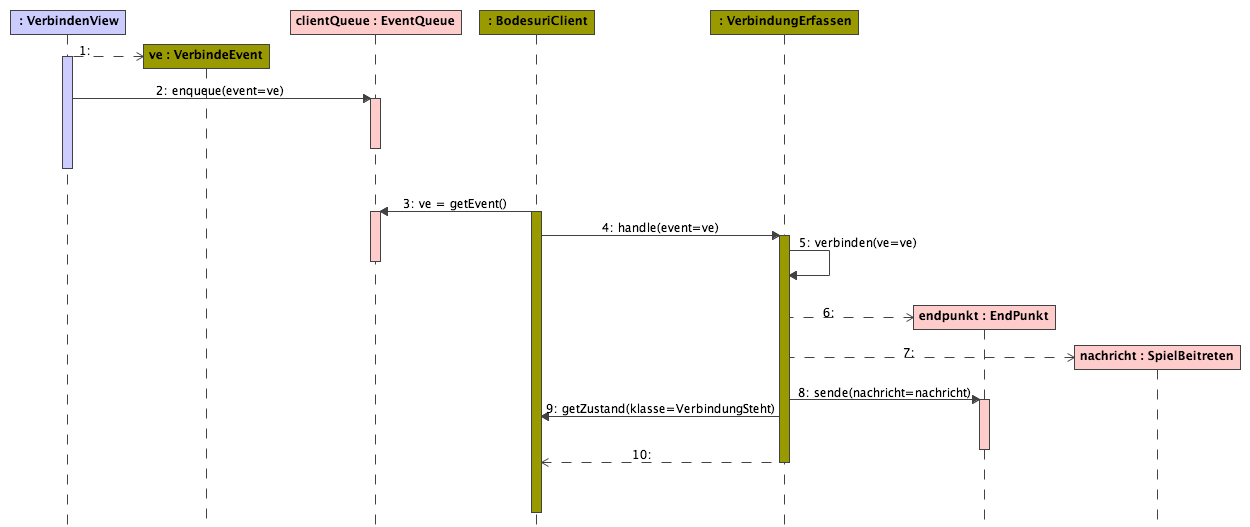
\includegraphics[width=\textwidth]{sd_verbindung_erstellen_client}
	\caption{Sequenzdiagramm Verbindung erstellen -- Client}
	\label{fig:sd_verbindung_erstellen_client}
\end{figure}
\begin{figure}[h]
	\centering
	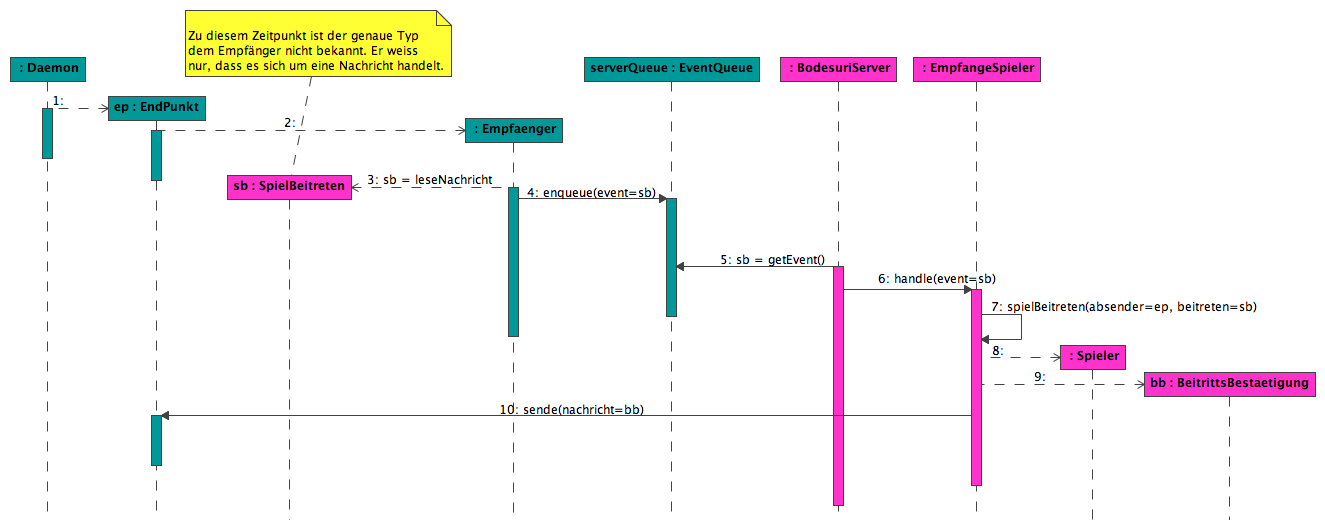
\includegraphics[width=\textwidth]{sd_verbindung_erstellen_server}
	\caption{Sequenzdiagramm Verbindung erstellen -- Server}
	\label{fig:sd_verbindung_erstellen_server}
\end{figure}

\begin{figure}[h]
	\centering
	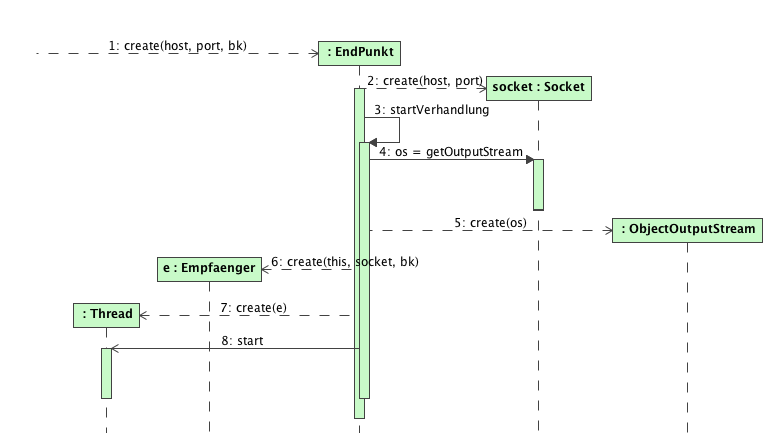
\includegraphics[width=\textwidth]{sd_verbindung_erstellen_endpunkt}
	\caption{Sequenzdiagramm Verbindung erstellen -- EndPunkt}
	\label{fig:sd_verbindung_erstellen_endpunkt}
\end{figure}

% subsection nachrichtenfluss_durch_die_schichten (end)

\subsection{Rundenstart} % (fold)
\label{sub:rundenstart}
Die Abbildung~\vref{fig:dienste_rundenstart} zeigt den Ablauf beim Start einer neuen Runde.
\begin{figure}[h]
	\centering
	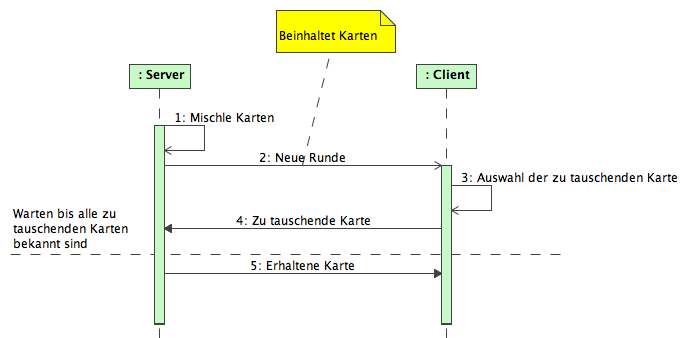
\includegraphics[width=0.7 \textwidth]{dienste_rundenstart}
	\caption{Sequenzdiagramm Rundenstart}
	\label{fig:dienste_rundenstart}
\end{figure}
% subsection rundenstart (end)

\clearpage
\subsection{Validierung von Spielzügen} % (fold)
\label{ssub:validierung_von_spielzügen}
Abbildung~\vref{fig:pd_validierung} zeigt die Validierung der Spielzüge.
\begin{figure}[h]
	\centering
	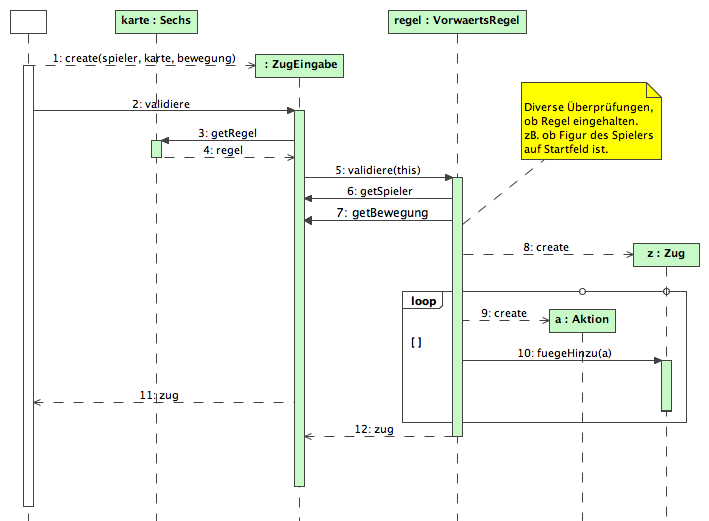
\includegraphics[width=\textwidth]{pd_validierung}
	\caption{Sequenzdiagramm Validierung von Spielzügen}
	\label{fig:pd_validierung}
\end{figure}
% subsection validierung_von_spielzügen (end)

\clearpage
\subsection{Serialiserung} % (fold)
\label{sub:serialiserung}
Abbildung~\vref{fig:dienste_serialisierung} zeigt den Ablauf bei der Serialisierung von Objekten, damit sie über das Netzwerk übertragen werden können.
\begin{figure}[h]
	\centering
	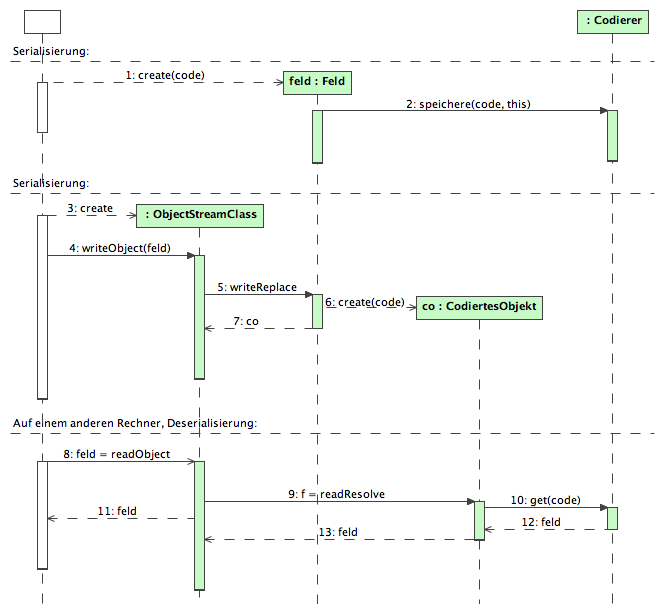
\includegraphics[width=\textwidth]{dienste_serialisierung}
	\caption{Sequenzdiagramm Serialisierung}
	\label{fig:dienste_serialisierung}
\end{figure}
% subsection serialiserung (end)

\clearpage
\subsection{Partnerschaften bilden} % (fold)
\label{sub:partnerschaften_bilden}
Abbildung~\vref{fig:dienste_partner} zeigt die möglichen Zustände beim Finden eines Partners.
\begin{figure}[h]
	\centering
	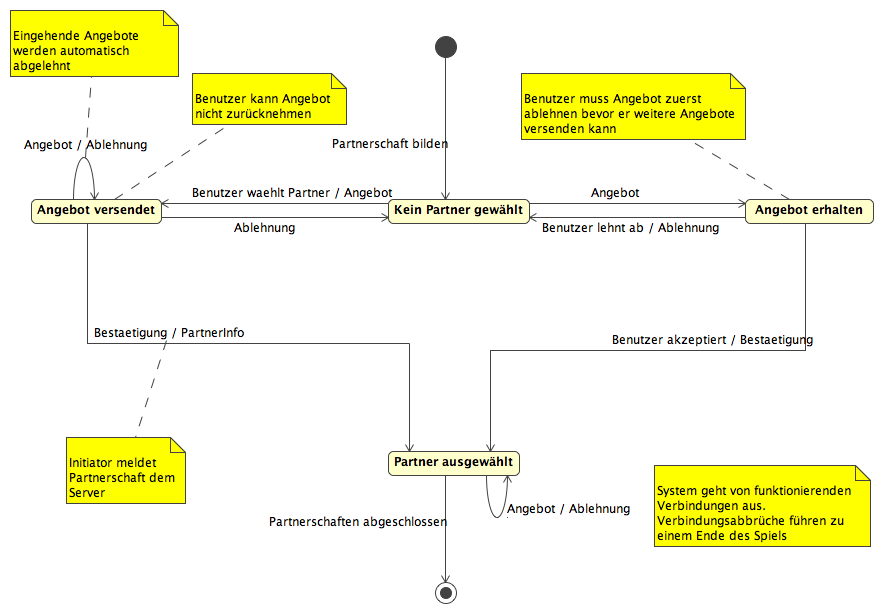
\includegraphics[width=\textwidth]{dienste_partner}
	\caption{Zustandsdiagramm Partnerschaften bilden}
	\label{fig:dienste_partner}
\end{figure}

Die Abildung~\vref{fig:dienste_partnerschaft_normal} zeigt Ablauf des Bildens von Partnerschaften.
\begin{figure}[h]
	\centering
	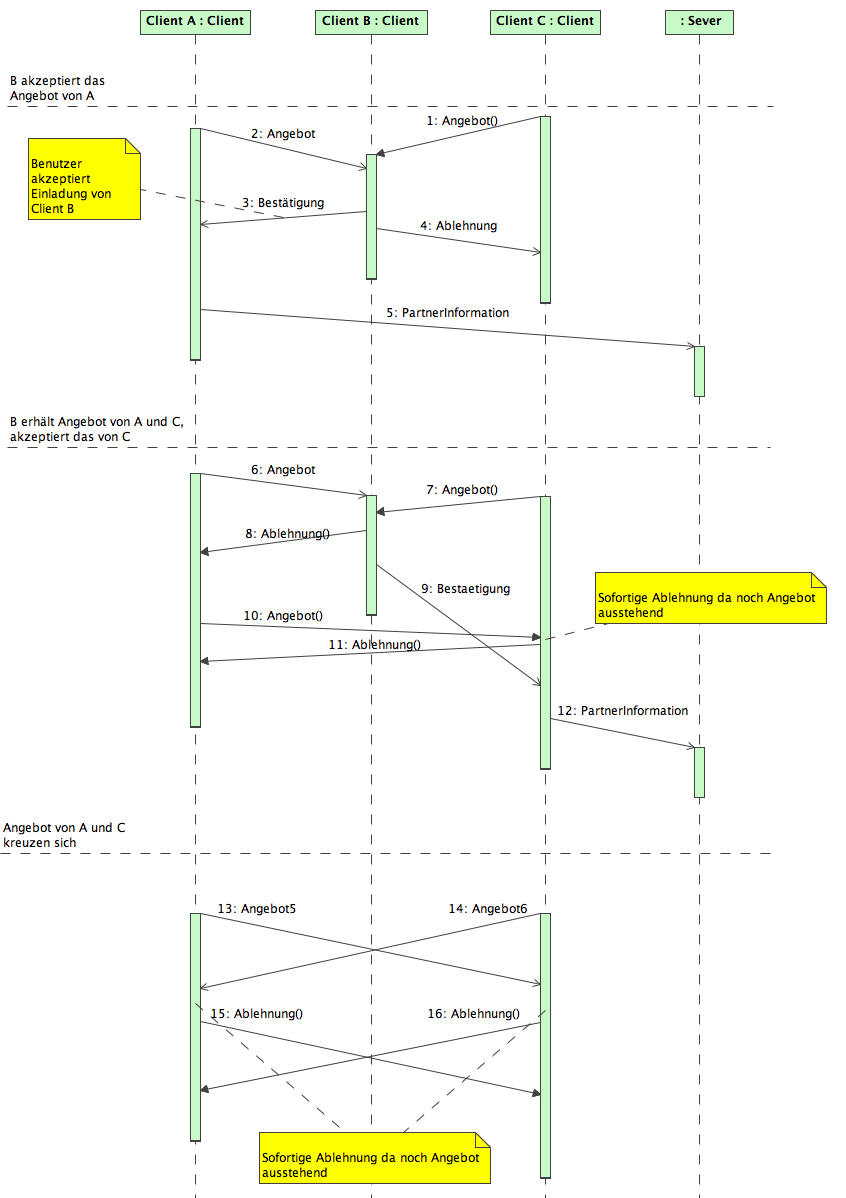
\includegraphics[width=\textwidth]{dienste_partnerschaft_normal}
	\caption{Sequenzdiagramm Partnerschaften bilden}
	\label{fig:dienste_partnerschaft_normal}
\end{figure}
% subsection partnerschaften_bilden (end)

\clearpage
\subsection{Chat} % (fold)
\label{sub:nachrichtenaustausch_zwischen_client_und_server}
Abbildung~\vref{fig:dienste_chat} zeigt den Verlauf des Austausches von Nachrichten zwischen den Clients und dem Server am Beispiel einer Chat-Nachricht.
\begin{figure}[h]
	\centering
	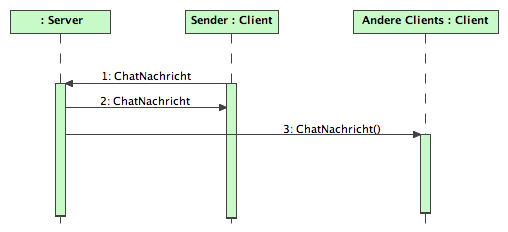
\includegraphics[width=\textwidth]{dienste_chat}
	\caption{Sequenzdiagramm Chat}
	\label{fig:dienste_chat}
\end{figure}
% subsection nachrichtenaustausch_zwischen_client_und_server (end)
\clearpage

\section{Externes Design} % (fold)
\label{externes_design}

\subsection{Verbinden}

Beim Starten des Spiels wird der Spieler aufgefordert, die Serverdaten zur Verbindung und seinen Spielernamen einzugeben.

\begin{figure}[h]
	\centering
	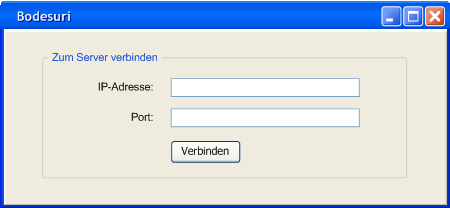
\includegraphics[width=0.7 \textwidth]{gui_verbindung}
	\caption{Design Verbinden}
	\label{fig:gui_verbindung}
\end{figure}

\clearpage

\subsection{Lobby} % (fold)
\label{externes_design_lobby}

In der Lobby können die Spieler einen Partner für das Spiel auswählen. Der ausgewählte Partner muss die Anfrage akzeptieren, um die Gruppe zu bilden. Sobald der Spieler bereit ist, das Spiel zu beginnen, wählt er im Spielstatus "<bereit"> aus. In der Zwischenzeit können sich die Spieler im Chat unterhalten.

\begin{figure}[h]
	\centering
	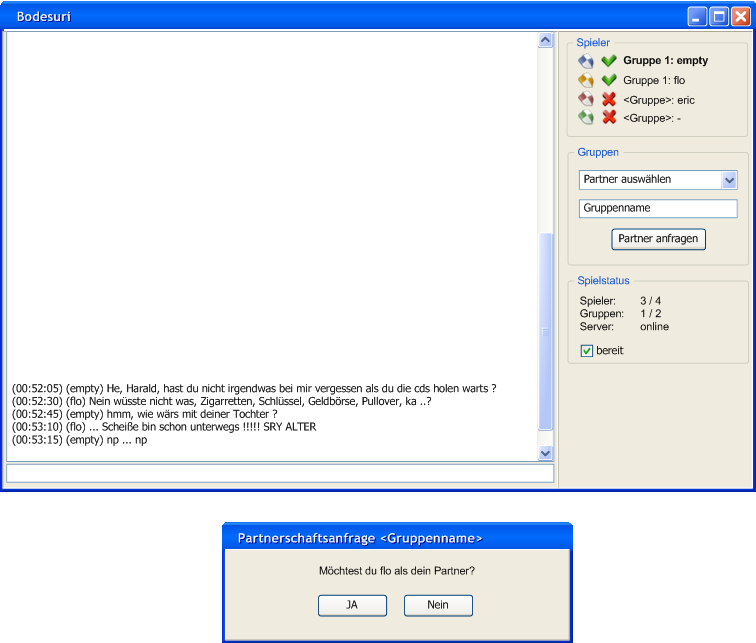
\includegraphics[width=0.9 \textwidth]{gui_lobby}
	\caption{Design Lobby}
	\label{fig:gui_lobby}
\end{figure}

\clearpage

\subsection{Spiel} % (fold)
\label{externes_design_spielbrett}

Das Spiel besteht aus verschiedenen Views:
\begin{itemize}
	\item In der BrettView wird das Spielbrett mit den Feldern und Spielfiguren dargestellt.
	\item In der SpielerView werden die einzelnen Spieler mit Gruppenzugehörigkeit aufgelistet.
	\item Die KartenView beinhaltet die Karten des Spielers.
	\item In der ChatView können sich die Spieler unterhalten.
\end{itemize}

\begin{figure}[h]
	\centering
	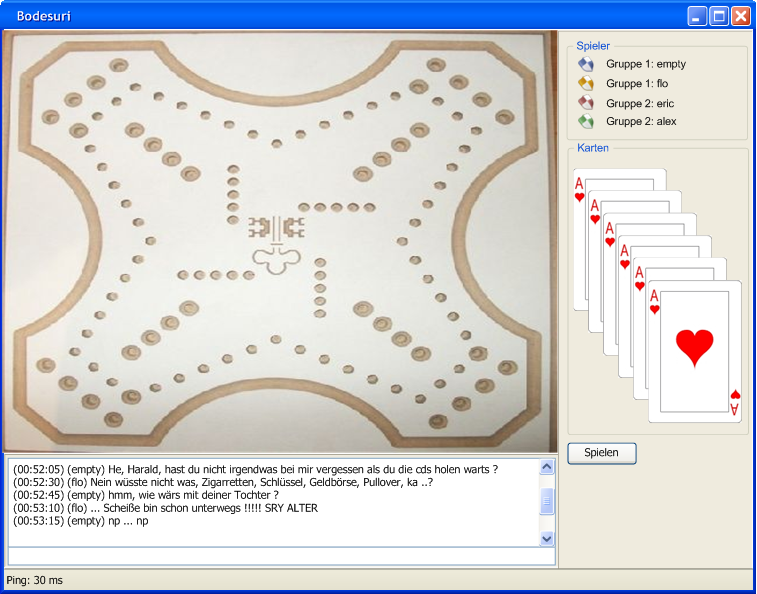
\includegraphics[width=0.9 \textwidth]{gui_spiel}
	\caption{Design Spiel}
	\label{fig:gui_spiel}
\end{figure}

% subsection externes_design (end)

\clearpage
\section{Eingetretene Risiken} % (fold)
\label{eingetretene_risiken}

\subsection{RMI} % (fold)
\label{sub:rmi}

Im Verlauf der ersten Tests mit RMI stellte sich schnell heraus, dass RMI weit mehr kann als für das Projekt notwendig wäre und es dem Projekt somit unnötig Komplexität hinzufügt. Andererseits stellt RMI  einige Anforderungen an die Client/Server-Struktur, die sich nur schwer mit den Projektanforderungen decken lassen. So kann RMI nur erschwert hinter Firewalls betrieben werden und eine Kommunikation über ein durch NAT\footnote{Network Adress Translation. Firewall-Feature welches Netzbereiche auf andere Netzbereiche abbildet. Wird häufig verwendet, um private Adressbereiche im Internet hinter einer einzelnen Adresse zu verstecken.} verstecktes Netzwerk ist gar nicht erst möglich. Da die Internet-Zugangslösungen in den meisten Haushalten auf Firewalls und NAT basieren, könnte das Spiel von einem grösseren Teil der potenziellen Kundschaft gar nicht gespielt werden.

Wir entschieden uns auf Grund dieser Probleme, auf eine eigene Lösung umzusteigen, welche auf den Java-Klassen Socket und Object(Input|Output)Stream basiert. Insgesamt gingen etwa 10 Stunden Arbeit für diese Umstellung verloren.
% subsection rmi (end)

\subsection{Java 2D} % (fold)
\label{java_2d}

Nachdem das CLI (Command Line Interface) erstellt war, entwarfen wir ein GUI dafür, das die Felder und Figuren darstellen sollte. Mit Java 2D ist das Zeichnen sehr einfach, da man die Koordinaten der zu zeichnenden Elemente angeben kann. Doch mussten wir leider feststellen, dass das Ansprechen eines Objektes etwas komplizierter ist. So muss zum Beispiel bei einem Mausklick das geklickte Objekt über die Koordinaten ermittelt werden. Ausserdem muss man sich um das Aktualisieren der Anzeige bei Veränderungen selber kümmern.

In einem zweiten Versuch erstellten wir das selbe Spielbrett mit Swing und wir kamen zum Schluss, dass dies die einfachere Methode ist. Die Objekte können mit einem speziellen Layout auch auf Koordinaten genau platziert werden und Klicke darauf kann man wie gewohnt mit einem MouseListener abfangen. Als Objekt kann man zum Beispiel ein Label mit einem Icon verwenden. Dies reicht für ein Brettspiel vollkommen aus.

Aus diesen Gründen haben wir uns dazu entschlossen, für das GUI als einzige Technologie Swing einzusetzen. Insgesamt gingen 7.5 Stunden Arbeit für diese Umstellung verloren.

% subsection java_2d (end)

% section eingetretene_risiken (end)

\listoffigures

\end{document}
